% this package is designed by: thanhhungqb@gmail.com
% more information and update: 
%   https://github.com/thanhhungqb/thesis-template
\documentclass[12pt,a4paper,oneside]{book} % twoside for draft

%\usepackage{babel}
\usepackage[utf8]{vietnam}
%\usepackage{times}
%\usepackage{graphicx}

\usepackage{mathptmx}	% same Time New Roma
%\renewcommand{\rmdefault}{phv} % Arial
%\renewcommand{\sfdefault}{phv} % Arial

\usepackage{fancyhdr}
\usepackage{algorithm2e}

\usepackage{bkthesis}

%\csdeptname{KHOA ĐIỆN ĐIỆN TỬ}
%\crname{BÁO CÁO THỰC TẬP TỐT NGHIỆP}
% \crname{BÁO CÁO TIỂU LUẬN}
\title{TÊN LUẬN VĂN / ĐỒ ÁN}
\cstuname{SVTH: Võ Thị Thuy}

\csCouncil{Khoa học máy tính}
\csSupervise{PGS. TS. Phạm Hồng Luân}
\csReviewer{TS. Pham Van Hai}
\cttime{1/2016}

\thesislayout

\begin{document}
%-	Bìa cứng - màu xanh dương, chữ mạ vàng (xem mẫu đính kèm)
%-	Trang tên (tờ lót): chất liệu giấy, nội dung giống như bìa LV
%-	Ở gáy LV: in nhan đề LV (có thể in tóm tắt nếu nhan đề quá dài), size 15 – 17
%-	Phiếu Nhiệm vụ LV, chấm điểm Hướng dẫn & Phản biện (đã ký): nhận từ GVHD & GVPB sau khi bảo vệ (theo lịch hẹn).
%-	Lời cam đoan
%-	Lời cảm ơn/ Lời ngỏ
%-	Tóm tắt LV
%-	Mục lục
%-	Danh mục, bảng biểu, hình ảnh, ... (nếu có)
%-	Nội dung LV
%-	Danh mục TL tham khảo
%-	Phụ lục (nếu có)

\coverpage

\frontmatter

% add content here
%-	Lời cam đoan
\begin{declaration}
	Tôi xin cam đoan...
\end{declaration}

%-	Lời cảm ơn/ Lời ngỏ
\begin{acknowledgments}
	Tôi xin chân thành cảm ơn ...
\end{acknowledgments}

%-	Tóm tắt LV
\begin{abstract}
	Tóm tắt luận văn ...
\end{abstract}	
	
\tableofcontents
%\listofsymbols
\listoftables
\listoffigures
%\listofalgorithms


\mainmatter

\fancyhead{}  % Clears all page headers and footers
%\rhead{\thepage}  % Sets the right side header to show the page number
%\lhead{}  % Clears the left side page header
%\fancyfoot[positions]{footer}
\renewcommand{\footrulewidth}{0.4pt}

\pagestyle{fancy}  % Finally, use the "fancy" page style to implement the FancyHdr headers


\chapter{Giới thiệu}
\section{Mở đầu}
Ngày nay sự phát triển không ngừng của công nghệ thông tin và truyền thông thông tin, điện thoại di động đã trở thành vật dụng không thể thiếu của hầu như tất cả mọi người.

Theo số liệu thống kê được công bố tại Ngày Internet Việt Nam 2015 do Hiệp hội Internet Việt Nam tổ chức tại Hà Nội 19/11/2015. Hiện nay, Việt Nam có 120 triệu thuê bao di động và theo sô liệu thu thập được từ công ty Appota liên quan đến lĩnh vực di động tại Việt Nam, hiện nay nước ta có khoảng 22 triệu người sử dụng smartphone tức là cứ 4 người Việt lại có 1 người sử dụng điện thoại thông minh, chiếm khoảng 19\% thuê bao di động.

Với một chiếc điện thoại di động, người dùng chẳng những có thể gọi điện, nhắn tin, phục vụ từ giải trí như: đọc tin tức (báo điện tử), nghe nhạc, xem phim, chơi game; cho đến đọc mail, viết ghi chú, và rất rất nhiều ứng dụng khác. Chính vì thế, chiếc điện thoại thông minh gần như là vật bất li thân của một bộ phân lớn người dùng.
 
Đi kèm với sự phát triển đó, một vấn nạn nảy sinh theo đó là tin nhắn rác \cite{ma2016}.

%Trong vài năm gần đây, tin nhắn rác thực sự là nỗi ám ảnh cho người dùng điện thoại di động. Cho dù cơ quan quản lý đã ra nhiều biện pháp xử lý nhưng vấn nạn này tiếp tục diễn ra và không có dấu hiệu suy giảm. Theo thống kê của công ty an ninh mạng BKAV, 6 tháng đầu năm 2015, tình hình phát tán tin nhắn rác không hề suy giảm mà tiếp tục gia tăng. Số lượng tin nhắn rác phát tán mỗi ngày lên tới 13.9 triệu tin, tăng hơn 0.4 triệu tin so với năm 2014. Ngoài ra, theo một thống kê khác của BKAV, khoảng 90\% thuê bao di động thường xuyên bị tin nhắn rác làm phiền, trong đó có 43\% là nạn nhân của các tin nhắn rác hằng ngày.

Với giá thành cho mỗi tin nhắn khá rẻ, chỉ khoảng 200vnđ cho mỗi tin nhắn nội mạng và 250vnđ cho mỗi tin nhắn ngoại mạng (giá thuê bao trả trước của nhà mạng mobifone).

Ngoài ra thì việc phát tán tin nhắn rác hàng loạt quá dễ dàng: có thể thông qua các đơn vị trung gian cung cấp dịch vụ phát tán tin nhắn rác dưới những cái tên như SMS marketing, tin nhắn marketing. Cước phí của dịch vụ này khá "phải chăng" như mạng Viettel - 45 đồng/tin, mạng Mobifone  - 40 đồng/tin, mạng VinaPhone - 27 đồng/tin. (Theo laodong.com.vn). Hoặc với các phần mềm gửi tin nhắn hàng loạt phổ biến như SMS Caster, TOP SMS Marketing, một cá nhân bình thường cũng có thể sử dụng và phát tán hàng nghìn tin nhắn chỉ với một cú click chuột.

Hơn nữa, hình phạt cho việc phát tán tin nhắn rác là rất nhẹ và sự bất lực của các nhà mạng trong vấn đề này khiến tin nhắn rác ngày một nhiều. Gây rất nhiều phiền toái cho người sử dụng.

Bắt đầu từ những vấn đề nêu trên, nhóm đã quyết định chọn đề tài: “Xây dựng bộ lọc tin nhắn rác cho điện thoại thông minh”. Đề tài nhằm mục đích xây dựng bộ lọc tin nhắn rác cho các tin nhắn tiếng Việt. Đáp ứng nhu cầu bức thiết của người sử dụng dịch vụ di động.

\section{Yêu cầu và mục tiêu của đề tài}

\subsection{Yêu cầu}

Nghiên cứu thuật toán phân loại tin nhắn rác.

Tạo ứng dụng chặn tin nhắn rác trên điện thoại thông minh (Android)

\subsection{Mục tiêu}

\subsubsection{Về kiến thức}

Phân tích, giải quyết yêu cầu bài toán phân loại tin nhắn rác

Nắm vững các thuật toán phân loại sử dụng

Nắm các kỹ thuật xử lý văn bản: tách token, tính xác suất các token,\ldots

Nắm các kiến thức lập trình di động (Android)

\subsubsection{Về sản phẩm}

Tối ưu hóa bộ lọc, ứng dụng

Nắm được quy trình phát triển sản phẩm: phân tích - thiết kế - hiện thực - kiểm tra.

Phát triển ứng dụng thực tế, hướng sử dụng, tương tác.

\section{Bố cục của luận văn}




%\input{demo-Chapter2.tex}
%\chapter{SYSTEM DESIGN}

\section{System architecture}
With the completion of system analysis, we are now 
focusing on designing the system architecture, how the system is organized and served to the end users. This section will 
discuss the detailed system architecture and services for deploying the system. As we 
can see from \textit{Figure 3.1}, the proposed architecture contains the 
following components:
\begin{figure}[H]
    \centering
    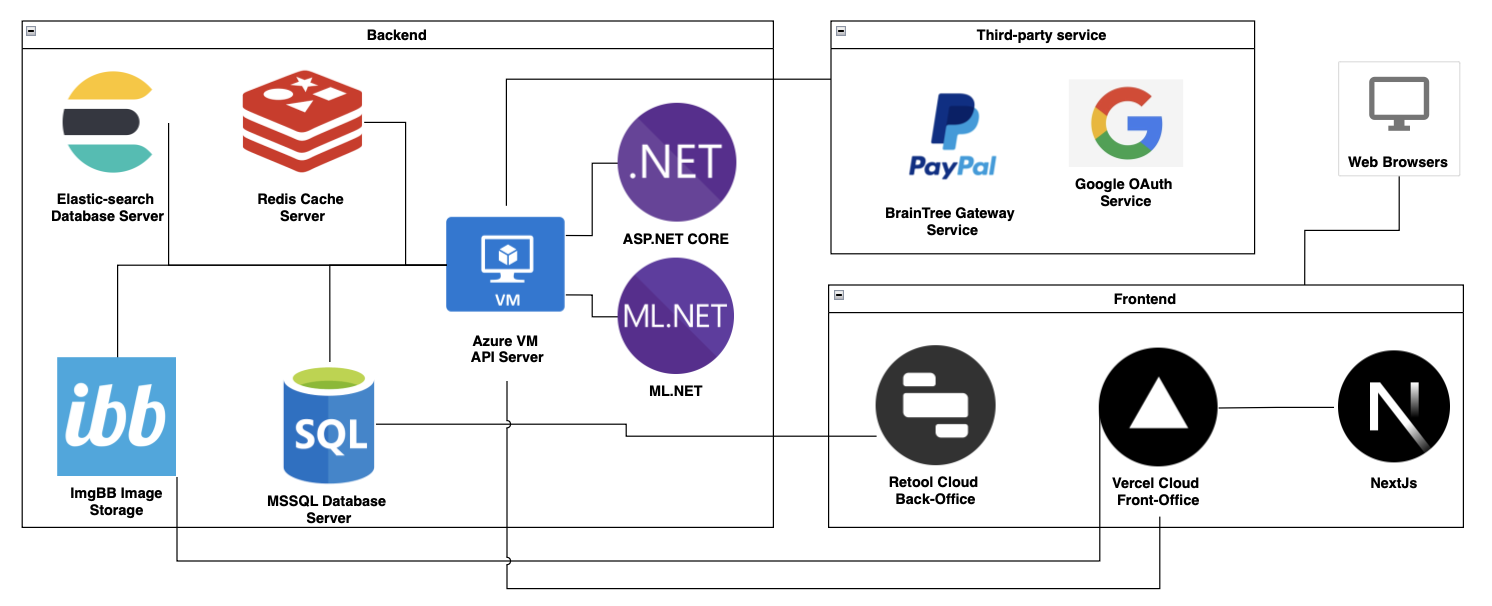
\includegraphics[width=1\textwidth]{Figures/Deployment/architect-report.png}
    \caption{Architecture Diagram}
    \label{fig:deployment-architecture}
\end{figure}
The Frontend component contains the back office and front office website of the system. This component is served to end users through web browsers.
\begin{itemize}
    \item \textit{Front office} handles user events and calls restful APIs from the API Server. It is implemented using Next.js and deployed on Vercel.
    \item \textit{Back office} is implemented using Retool. It interact directly to the MSSQL Database Server.
\end{itemize}

The backend of the system includes components as follows:
\begin{itemize}
    \item \textit{API Server} is the central part of the system, focusing on 
    handling all business logics and flows, serving API for the front office, 
    and interacting with other components of the system. It is implemented by ASP.NET Core and ML.NET and deployed by an Azure Virtual Machine.
    \item \textit{MSSQL Database Server} is the place where the database of the system is served. 
    This server interacts with the API Server and the back office.
    \item \textit{Imgbb Image Server} stores all the static images of the system. Images will 
    be uploaded directly from the front office to the Imgbb Image Server before storing the returned URLs in the SQL Database Server. This component will 
    be served by a free Imgbb cloud service.
    \item Furthermore, we will have two corresponding servers for caching data and optimizing 
    data search speed using a free \textit{Elastic-search cloud} and \textit{Azure Redis Cache Database}.
\end{itemize}

Finally, third-party services for authentication (Google OAuth Service) and payment (BrainTree Gateway Service) purposes are implemented by connecting to the API Server.

\section{UI/UX design}

In this section, we delve into the UI/UX design for our pet adoption website. Each page has been crafted to enhance user engagement and streamline the adoption process. Begins on the homepage, where users are welcomed with an intuitive interface that serves as the gateway to the platform. The login and register pages provide a seamless onboarding experience, ensuring a secure and personalized environment. The pet search page facilitates effortless exploration, allowing users to discover potential companions with ease. Detailed pet profiles showcase comprehensive information, fostering informed decision-making. The user profile page ensures a tailored experience, while the blog homepage and pages provide valuable insights and updates. To navigate this cohesive ecosystem, a diagram illustrates the interconnectedness of each page, illuminating the user's journey from entry to adoption. To enhance clarity, we've included a comprehensive diagram illustrating the intricate connections between these pages
\subsection{Front office}

\begin{figure}[H]
    \centering
    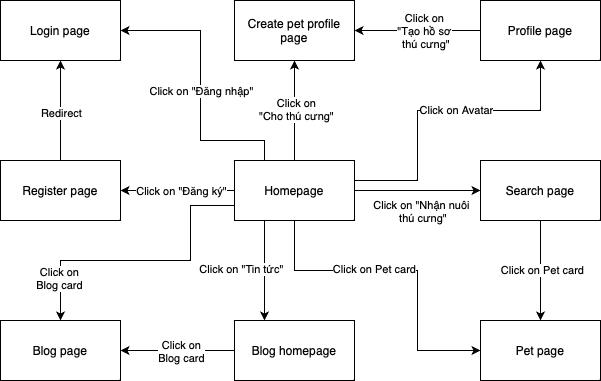
\includegraphics[width=0.8\textwidth]{Figures/wireframe_fo.png}
    \caption{Wireframe for Front office}
\end{figure}

\subsubsection{Homepage}

The homepage serves as the focal point of our pet adoption website, designed with a user-centric approach to ensure an intuitive and engaging experience. The navigation bar stands as a gateway to key functionalities, allowing users to seamlessly register, log in, explore pet profiles, create their pet profiles, access insightful blog content, and manage their user profile. The strategic placement of these navigation options facilitates effortless interaction. The hero section captures attention with visually appealing imagery and succinct messaging, encapsulating the essence of our mission. The "About Us" section provides a deeper understanding of our organization, building trust and connection with our audience. Additionally, the organization section offers insights into our partners and collaborators, fostering a sense of community.

\begin {figure}[H]
\centering
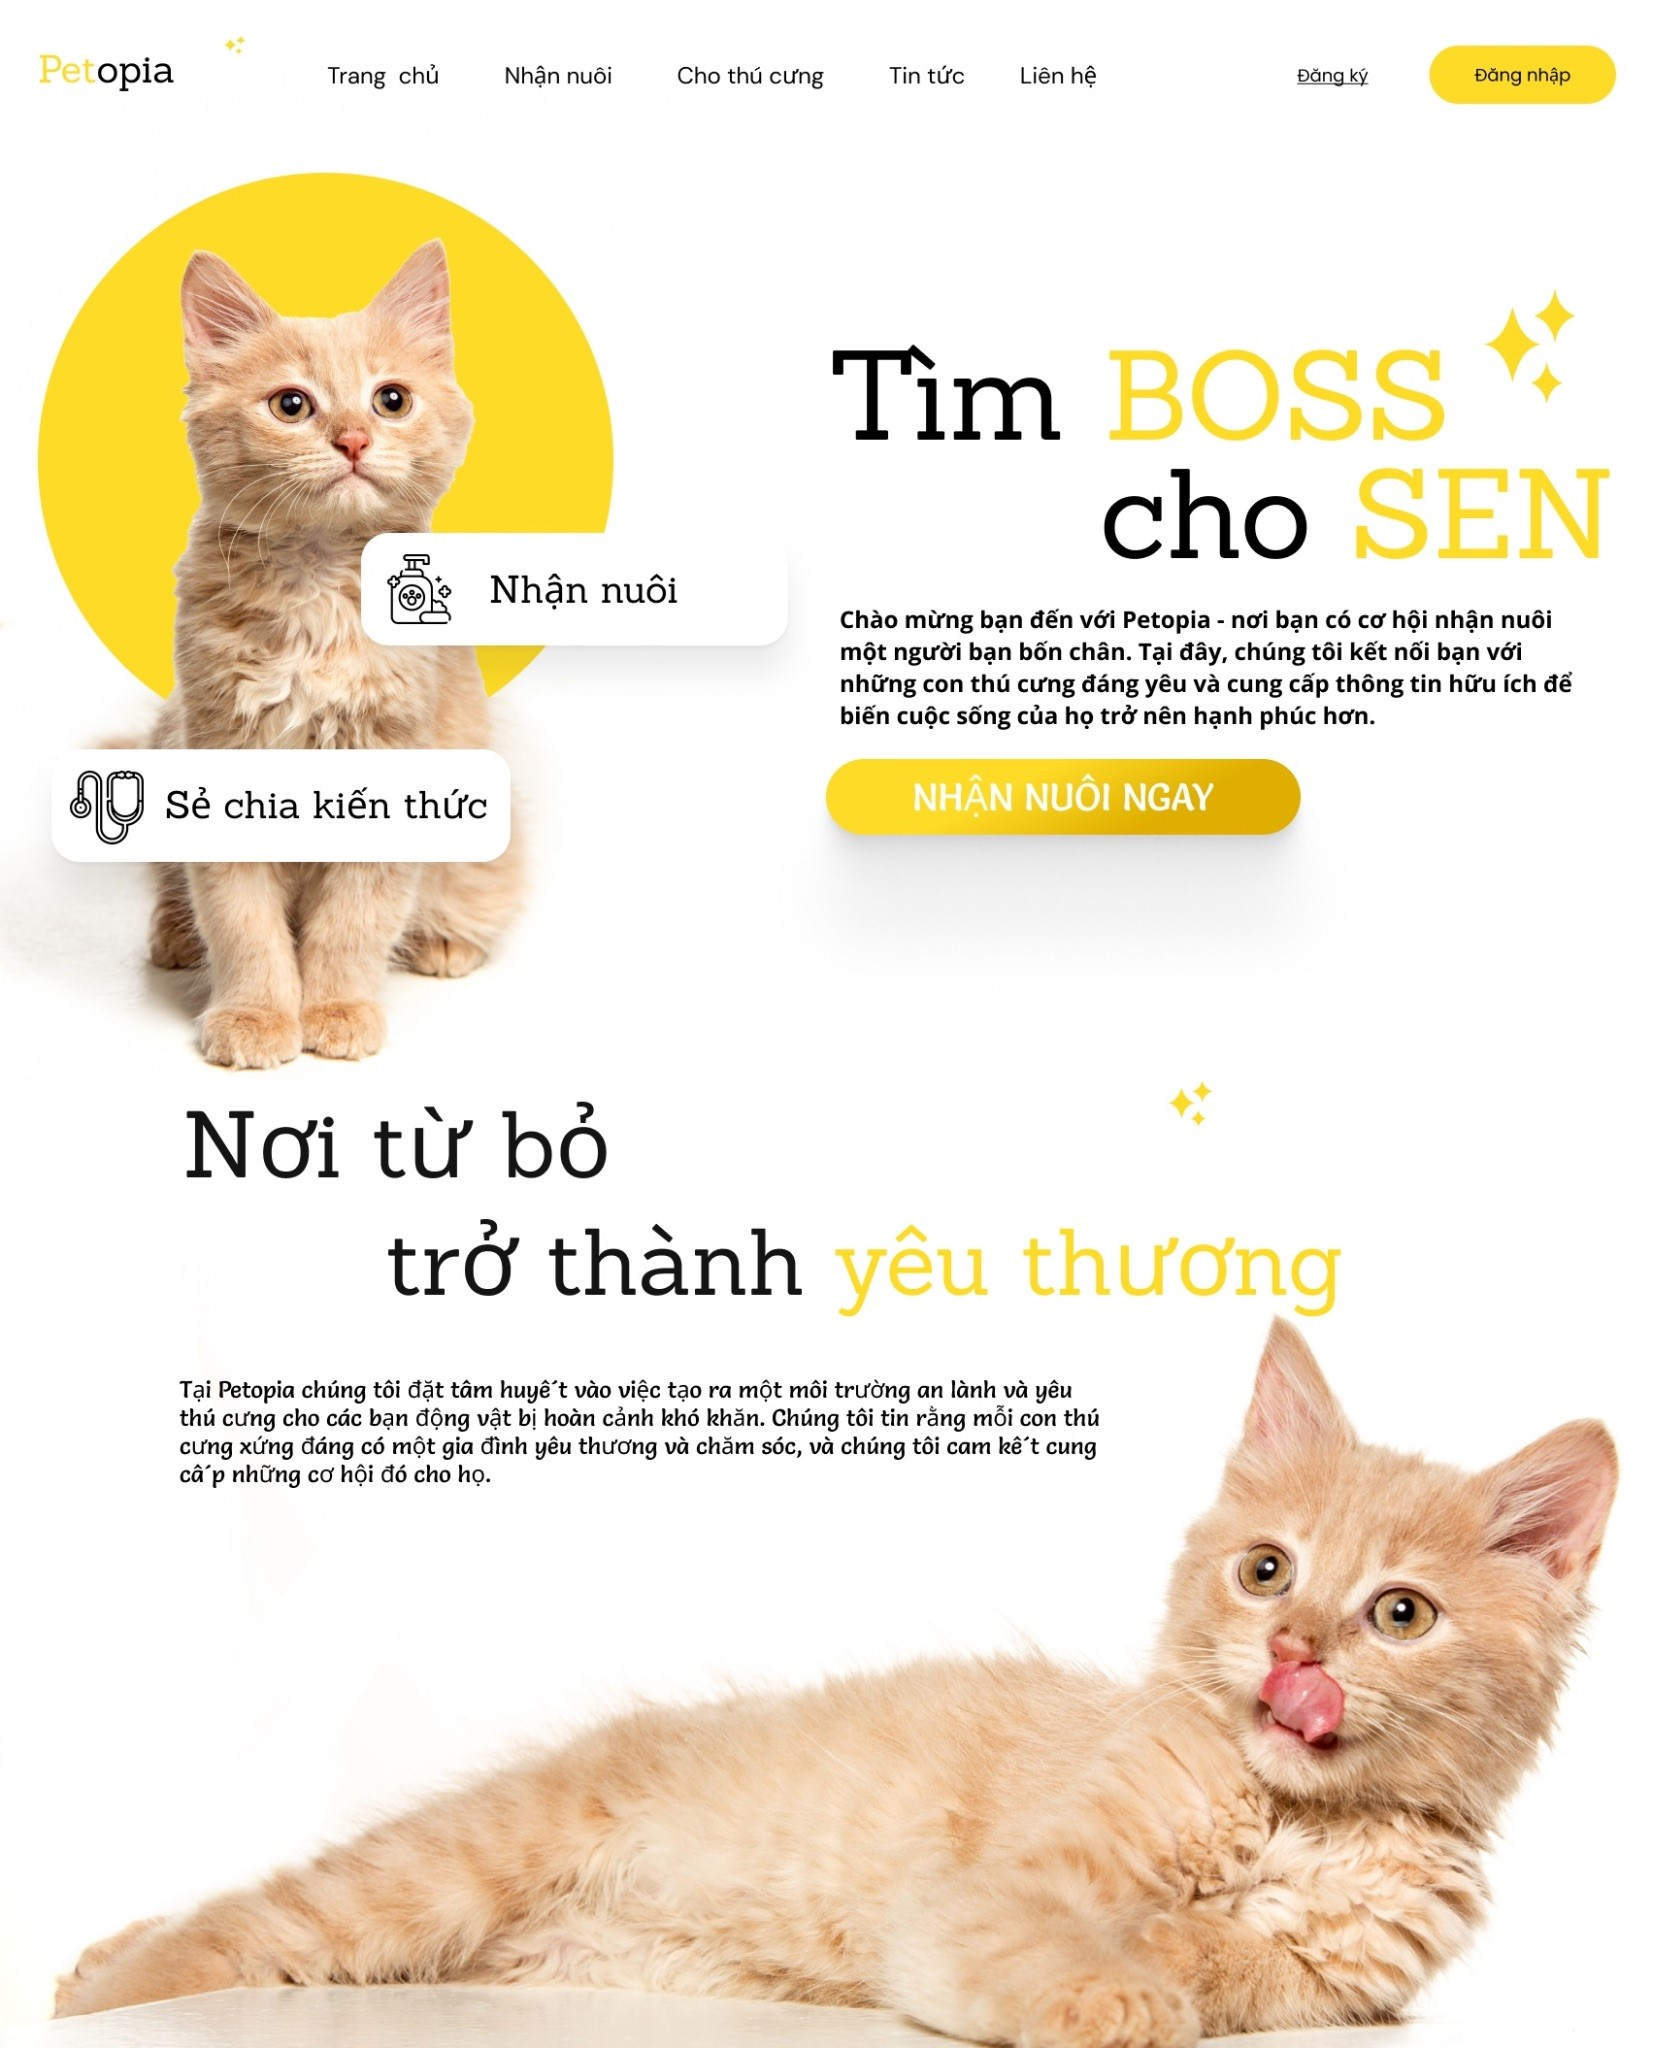
\includegraphics[width=0.8\textwidth]{Figures/UI/home_ui.jpg}
\caption{Homepage of Petopia}
\end{figure}

\subsubsection{Login}

Our homepage's login functionality is designed for simplicity and security, providing a seamless entry into the pet adoption experience. Users can access the login page with a click on the "Đăng nhập" button, where they input their Gmail and password. Error notifications guide users in case of issues, and a convenient register button directs new users to the registration page. For accessibility, users can also log in using their Google account, streamlining the process. A "Forgot Password" option is available for password resets, ensuring a hassle-free and secure experience that accommodates diverse user preferences.

\begin{figure}[H]
    \centering
    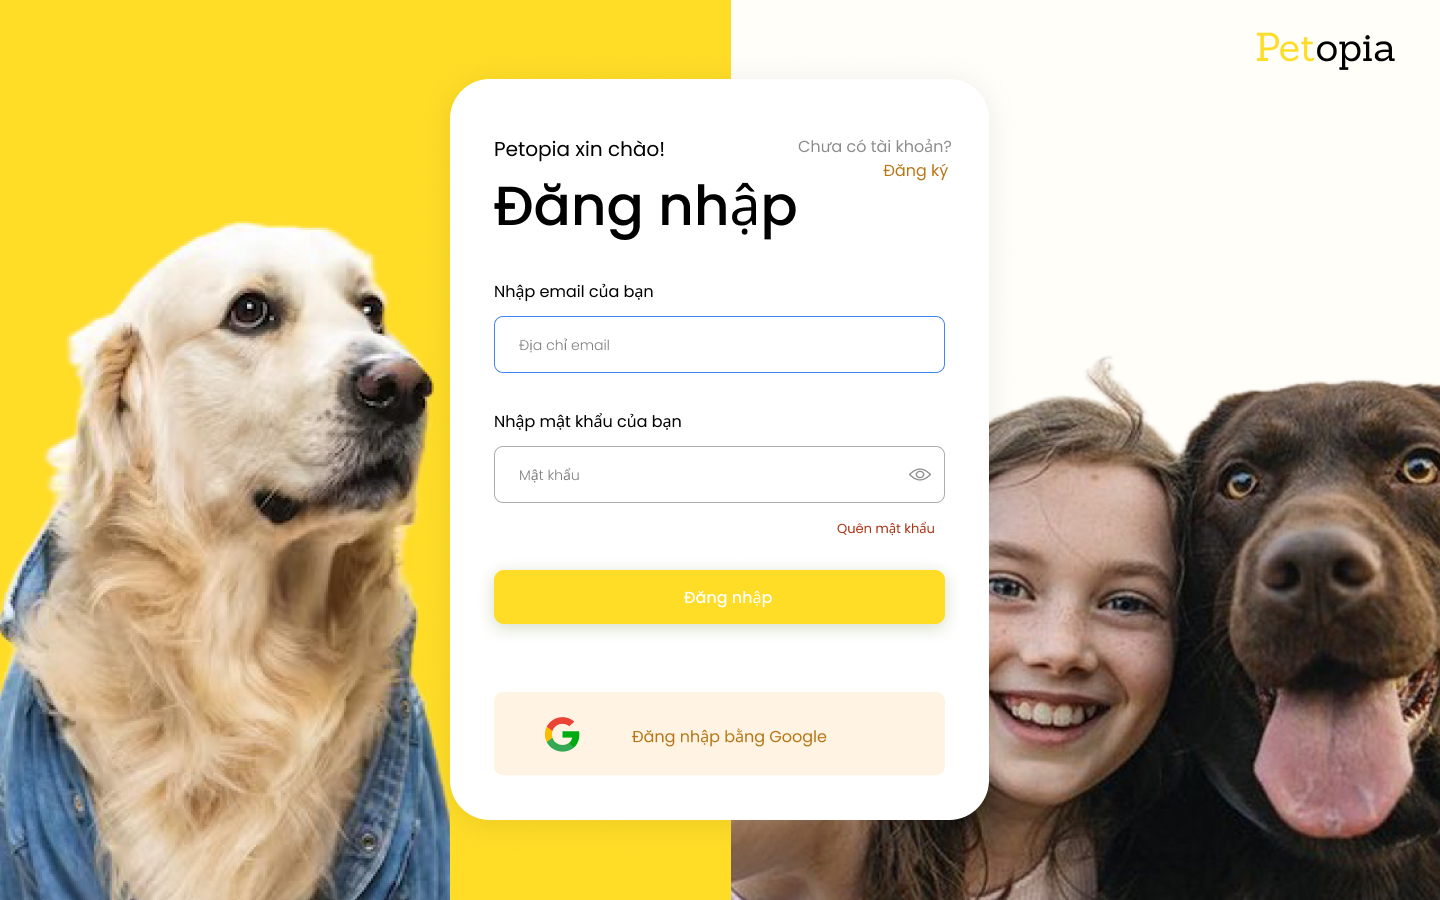
\includegraphics[width=0.8\textwidth]{Figures/UI/login_ui.png}
    \caption{Login form}
\end{figure}

\subsubsection{Register}

The registration process is straightforward, requiring users to input essential information such as first name, last name, Gmail, and password. After clicking "Register," the system verifies the form's completeness and prompts users to check their email for account verification. A verification link enhances security, ensuring authenticity. Clicking the link redirects users to the login page, confirming successful account creation. This two-step process prioritizes security and user-friendly guidance, fostering trust in our platform.

\begin{figure}[H]
    \centering
    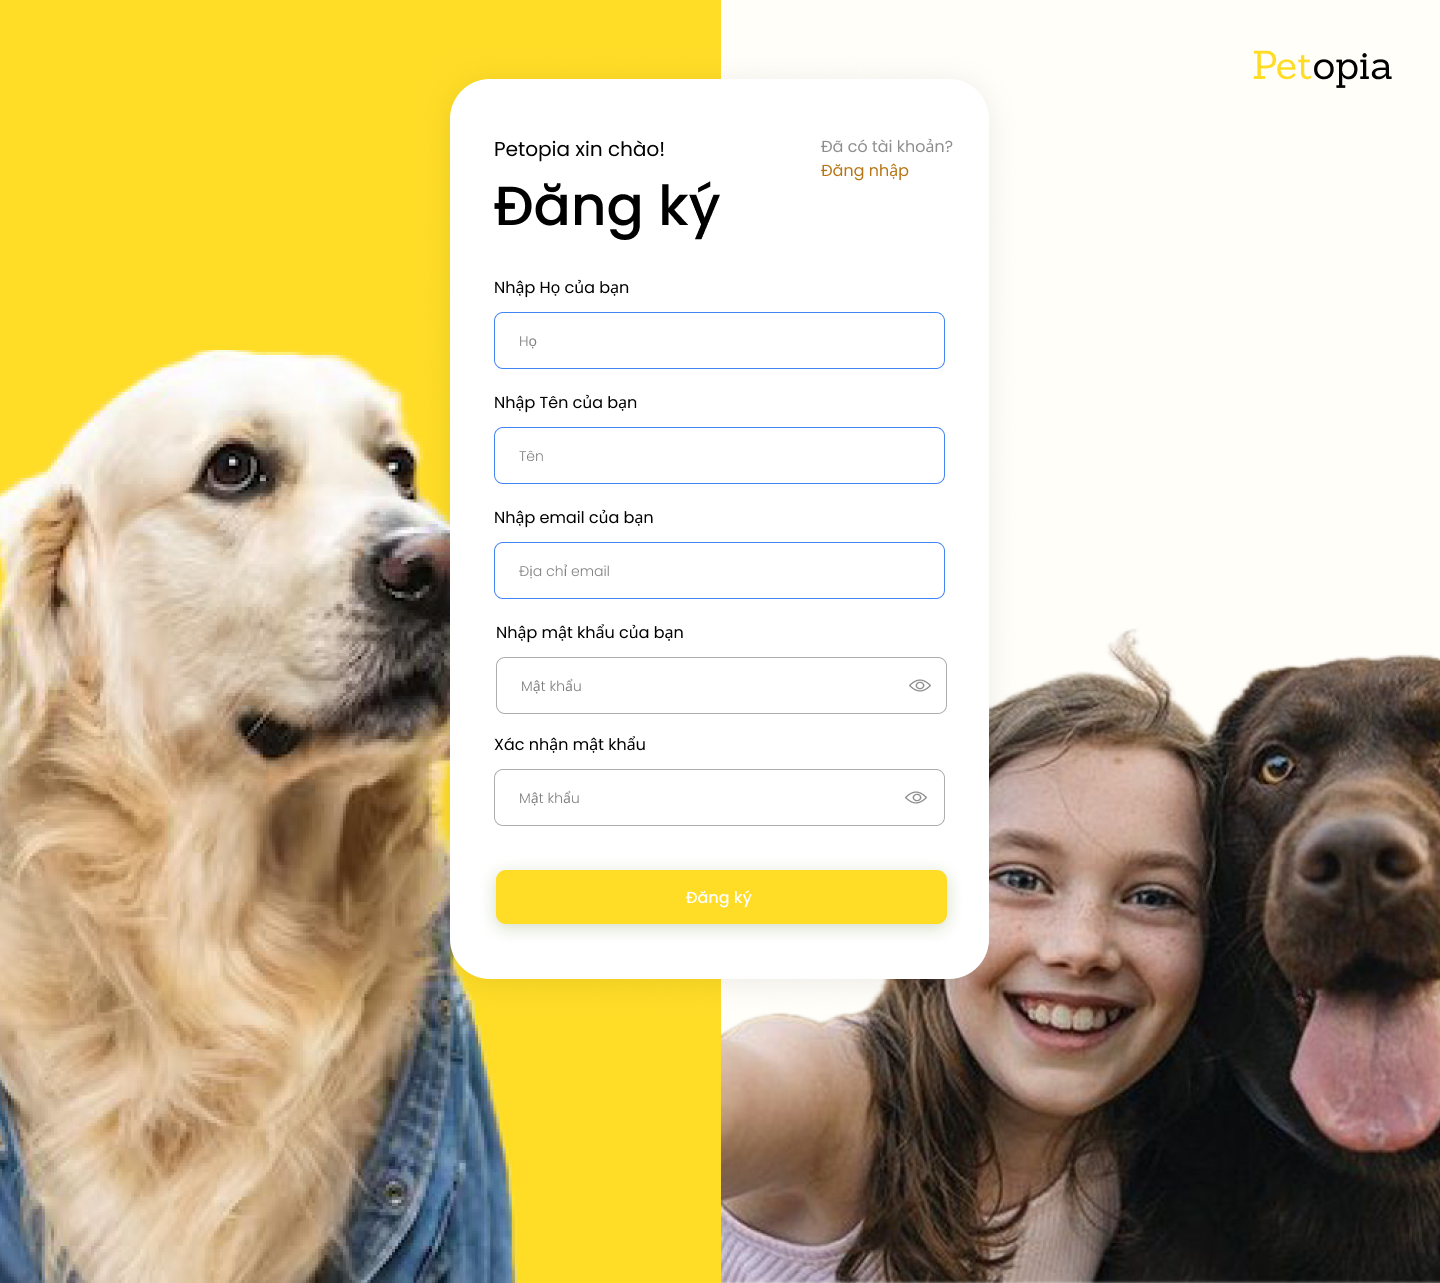
\includegraphics[width=0.5\textwidth]{Figures/UI/register_ui.png}
    \caption{Register form}
\end{figure}

\subsubsection{Search page}

The pet search page is designed for precision and ease. Users can tailor their search 
with checkboxes for sex, breed, color, size, and vaccination status. A sorting feature 
arranges results for flexibility. A prominent search bar, and supporting text and image
 queries, ensure a personalized and efficient experience. Robust filtering, sorting, and 
 versatile search methods aim to provide a user-friendly pet discovery journey on our platform.

\begin{figure}[H]
    \centering
    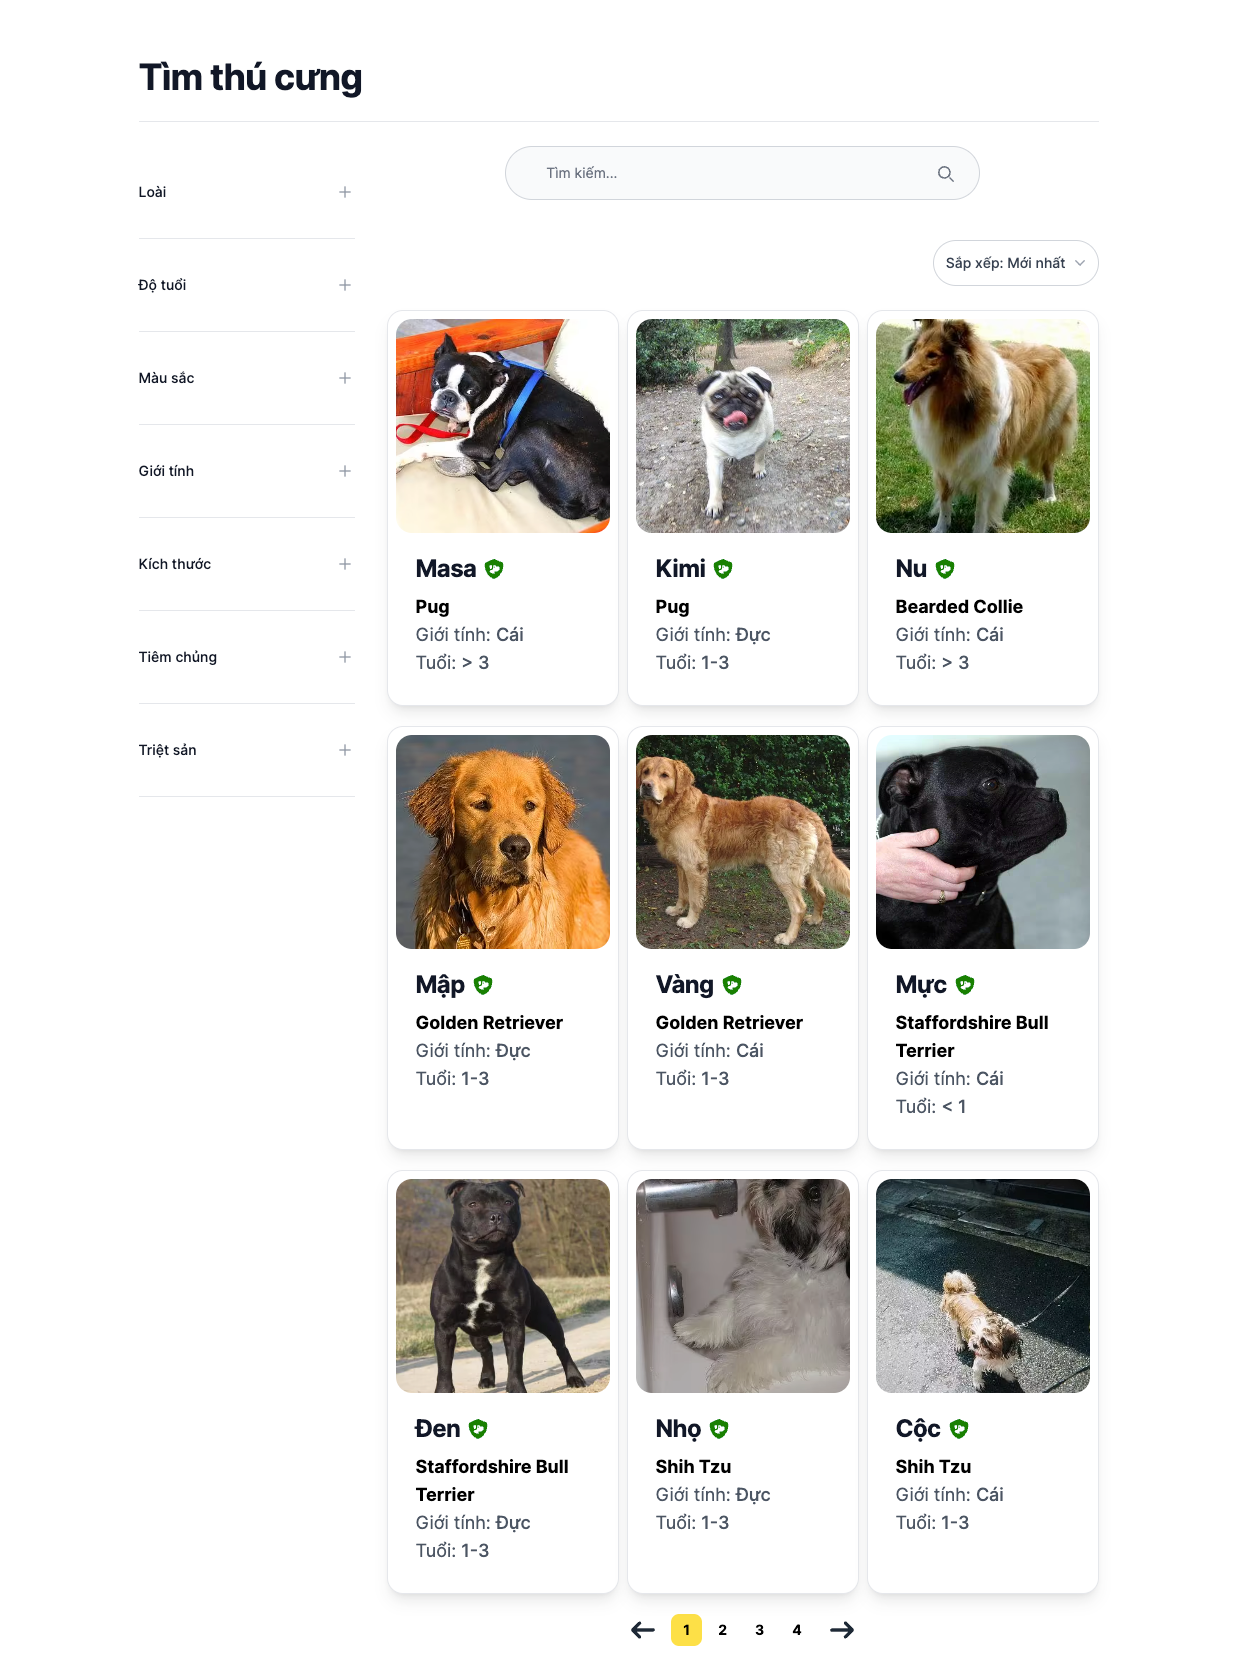
\includegraphics[width=0.8\textwidth]{Figures/UI/search_ui.png}
    \caption{Search page for searching desired pet}
\end{figure}


\subsubsection{Pet profile}

The pet page is a comprehensive showcase, providing detailed insights into each pet. Clicking on a pet card redirects users to the dedicated pet profile page, displaying key information such as name, breed, age, and vaccination status. Striking images and a personal description offer a deeper understanding of the pet's personality. A prominent "Adopt" button facilitates the adoption process, dynamically revealing an efficient adoption form upon click. This ensures transparent communication between potential adopters and pet owners.

\begin{figure}[H]
    \centering
    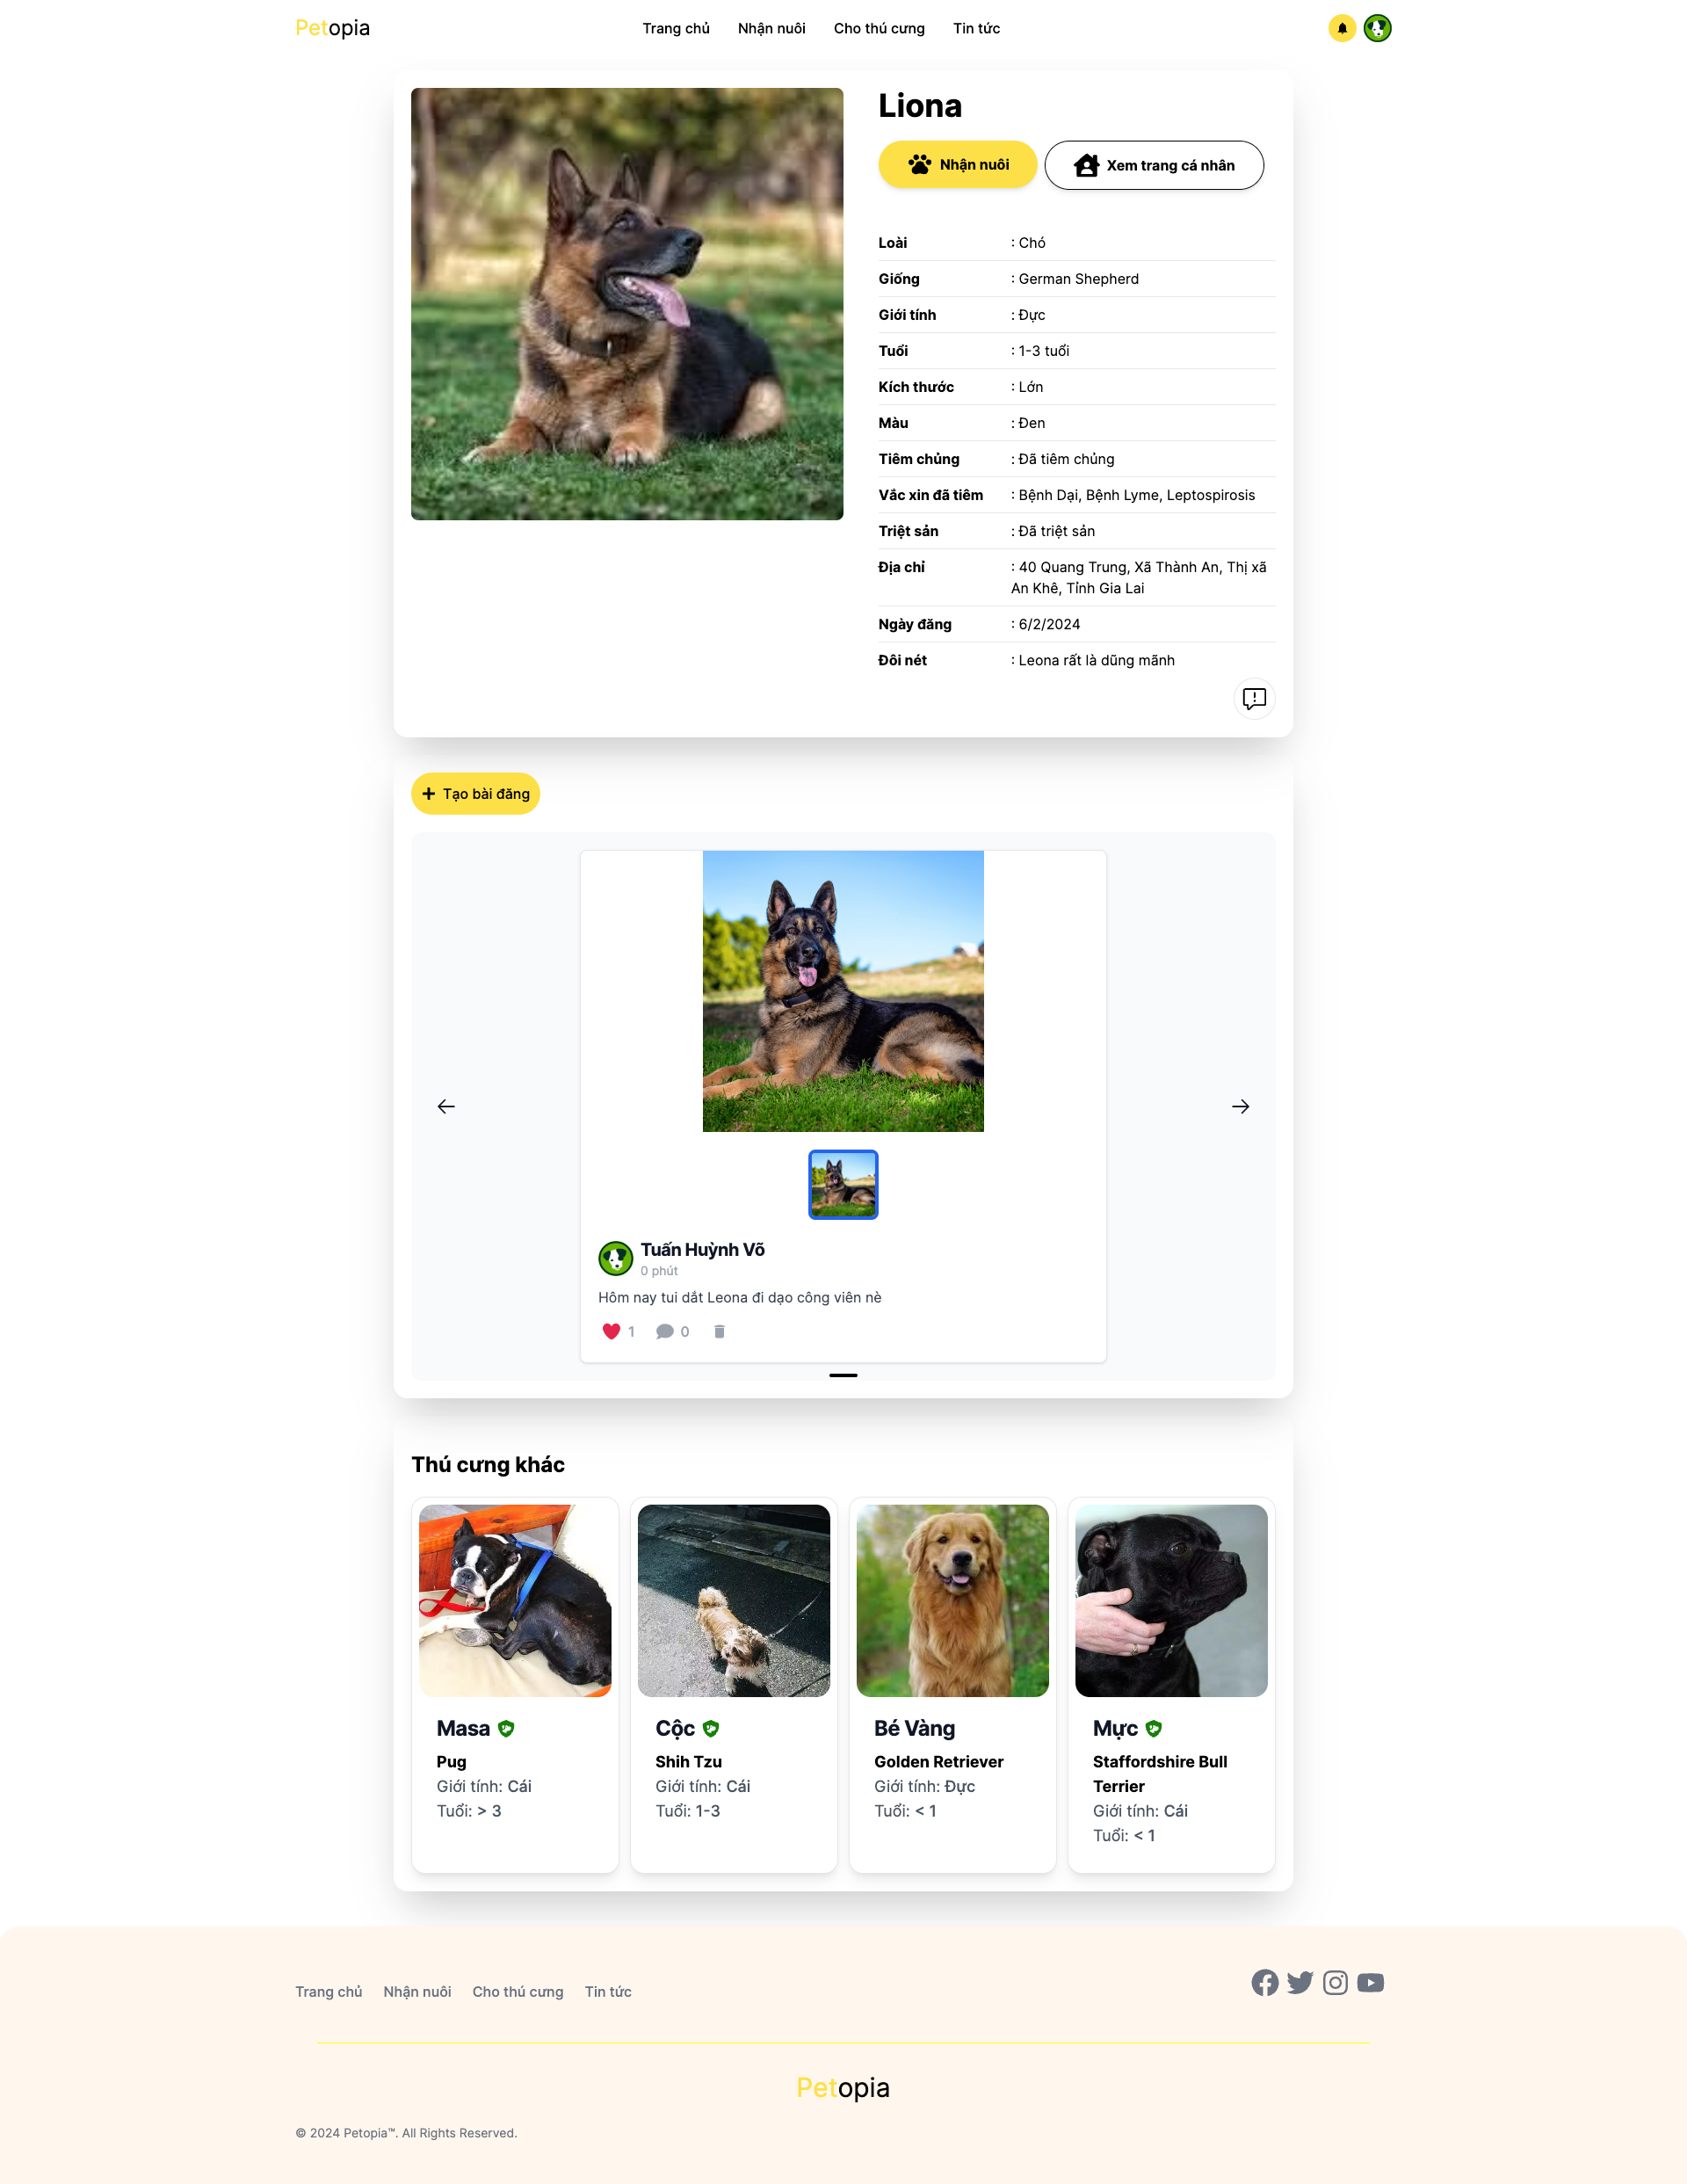
\includegraphics[width=0.6\textwidth]{Figures/UI/pet_detail_ui.png}
    \caption{Pet profile page}
\end{figure}

\subsubsection{Create pet profile}

\begin{figure}[H]
    \centering
    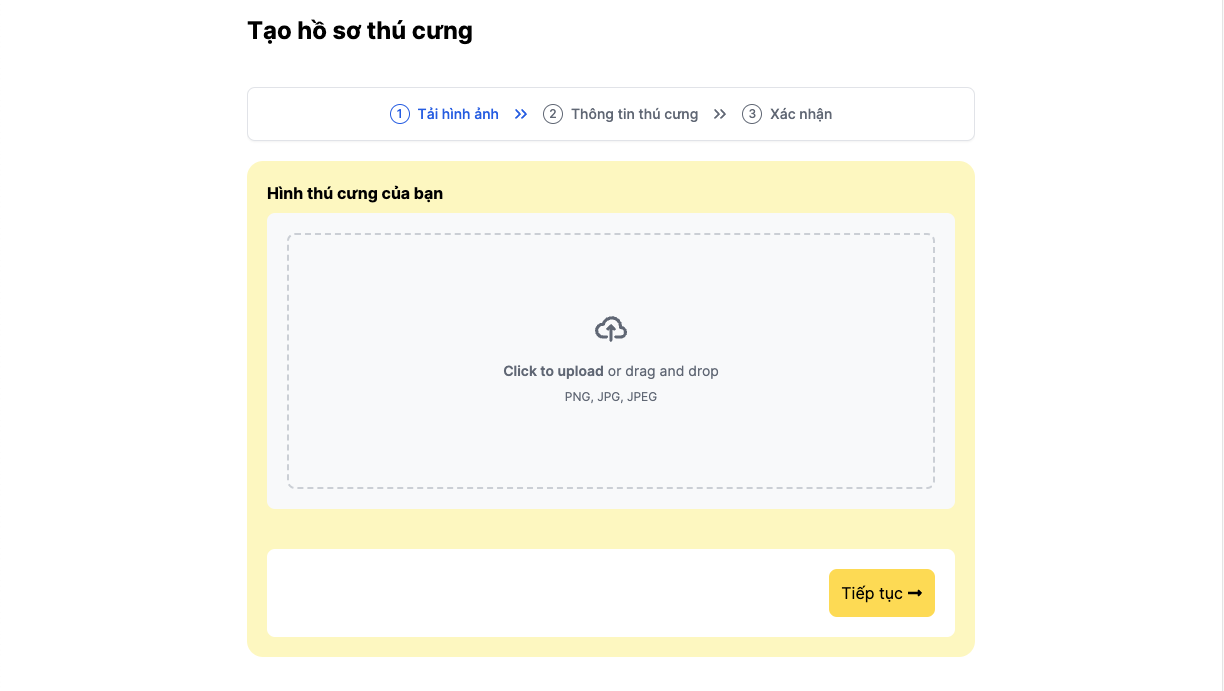
\includegraphics[width=0.6\textwidth]{Figures/UI/image_upload_ui.png}
    \caption{Image upload form}
\end{figure}

\begin{figure}[H]
    \centering
    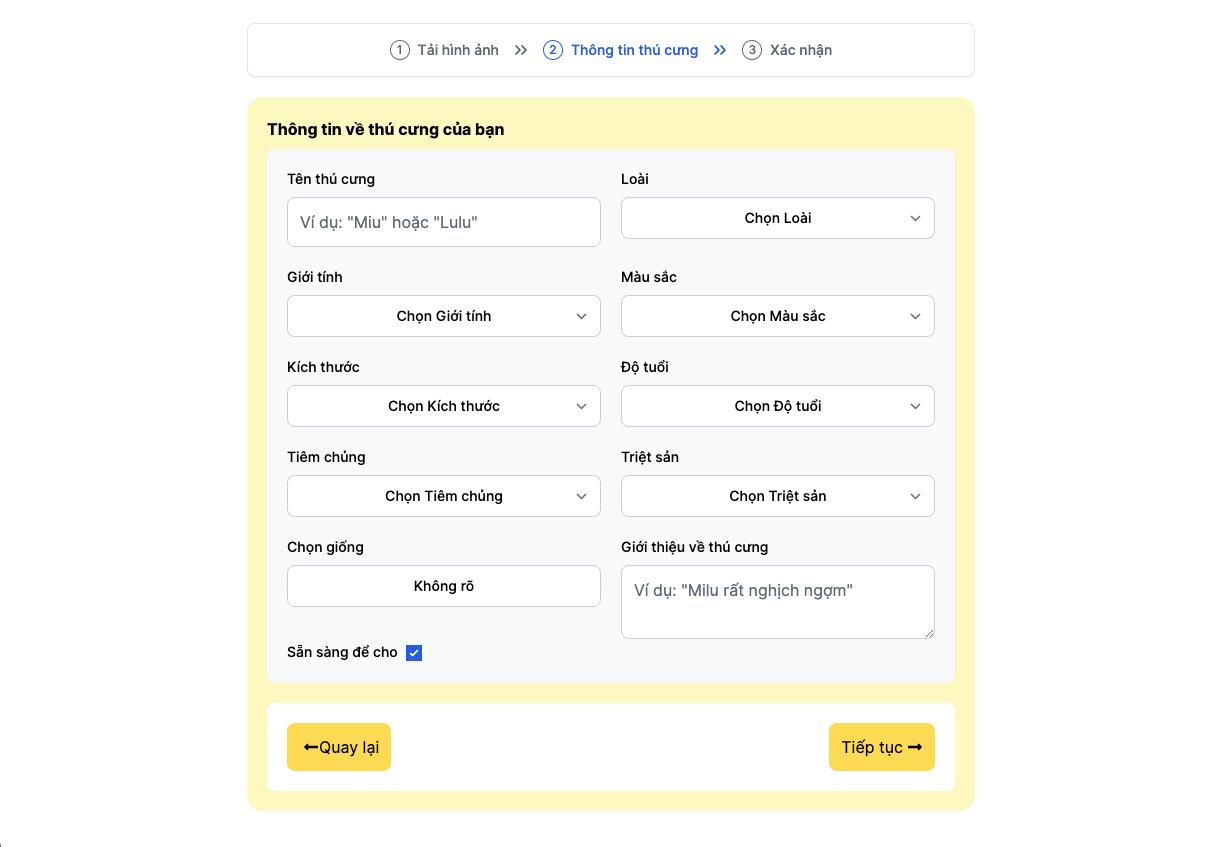
\includegraphics[width=0.6\textwidth]{Figures/UI/pet_input_ui.png}
    \caption{Form for taking user's pet detail}
\end{figure}

\begin {figure}[H]
\centering
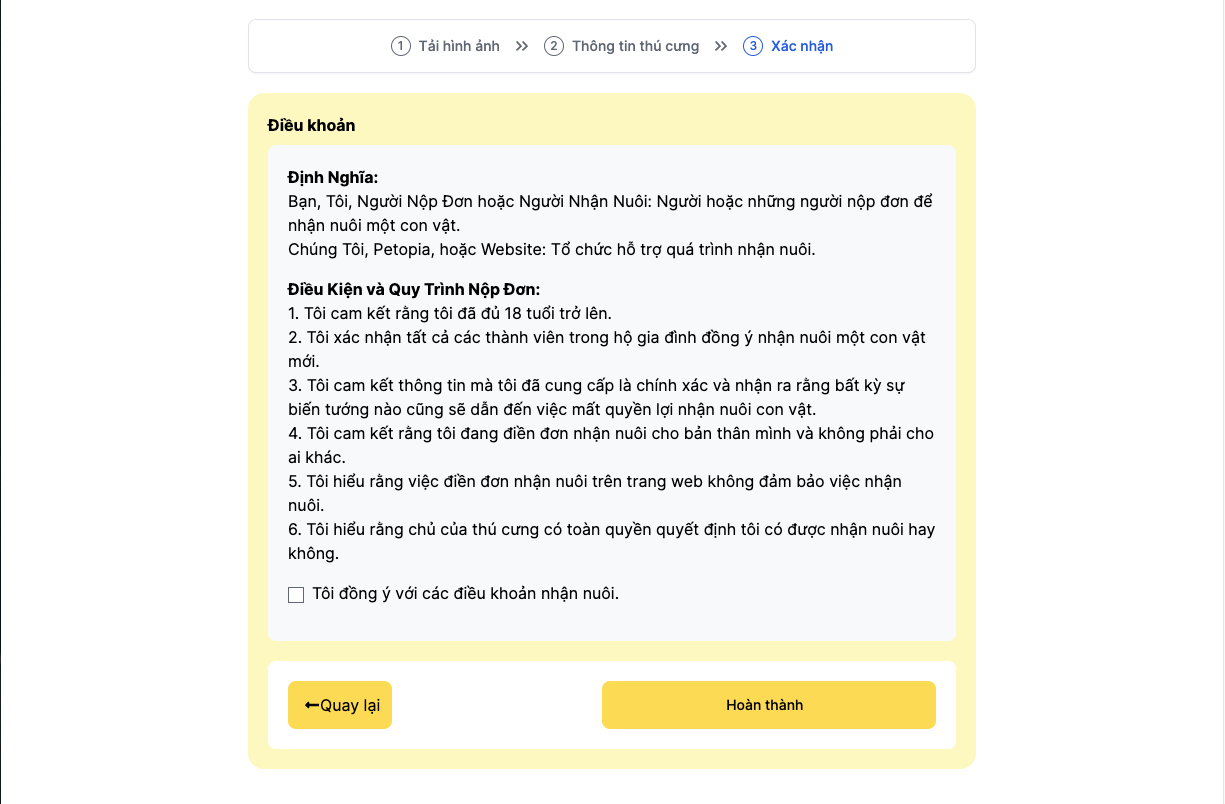
\includegraphics[width=0.6\textwidth]{Figures/UI/term_ui.png}
\caption{Pet profile page}
\end{figure}

Creating a pet profile on our platform is user-friendly and efficient. Users begin by uploading a pet image (Figure 3.8), which our AI processes to autofill the breed. Clicking "Continue" leads to a detailed pet form (Figure 3.9) for additional information. Users then review the Terms and Services (Figure 3.10) before clicking "Finish" to complete the profile. This structured process, with AI assistance in the initial steps, ensures accuracy and a seamless user experience.

\subsubsection{User profile}

\begin{figure}[H]
    \centering
    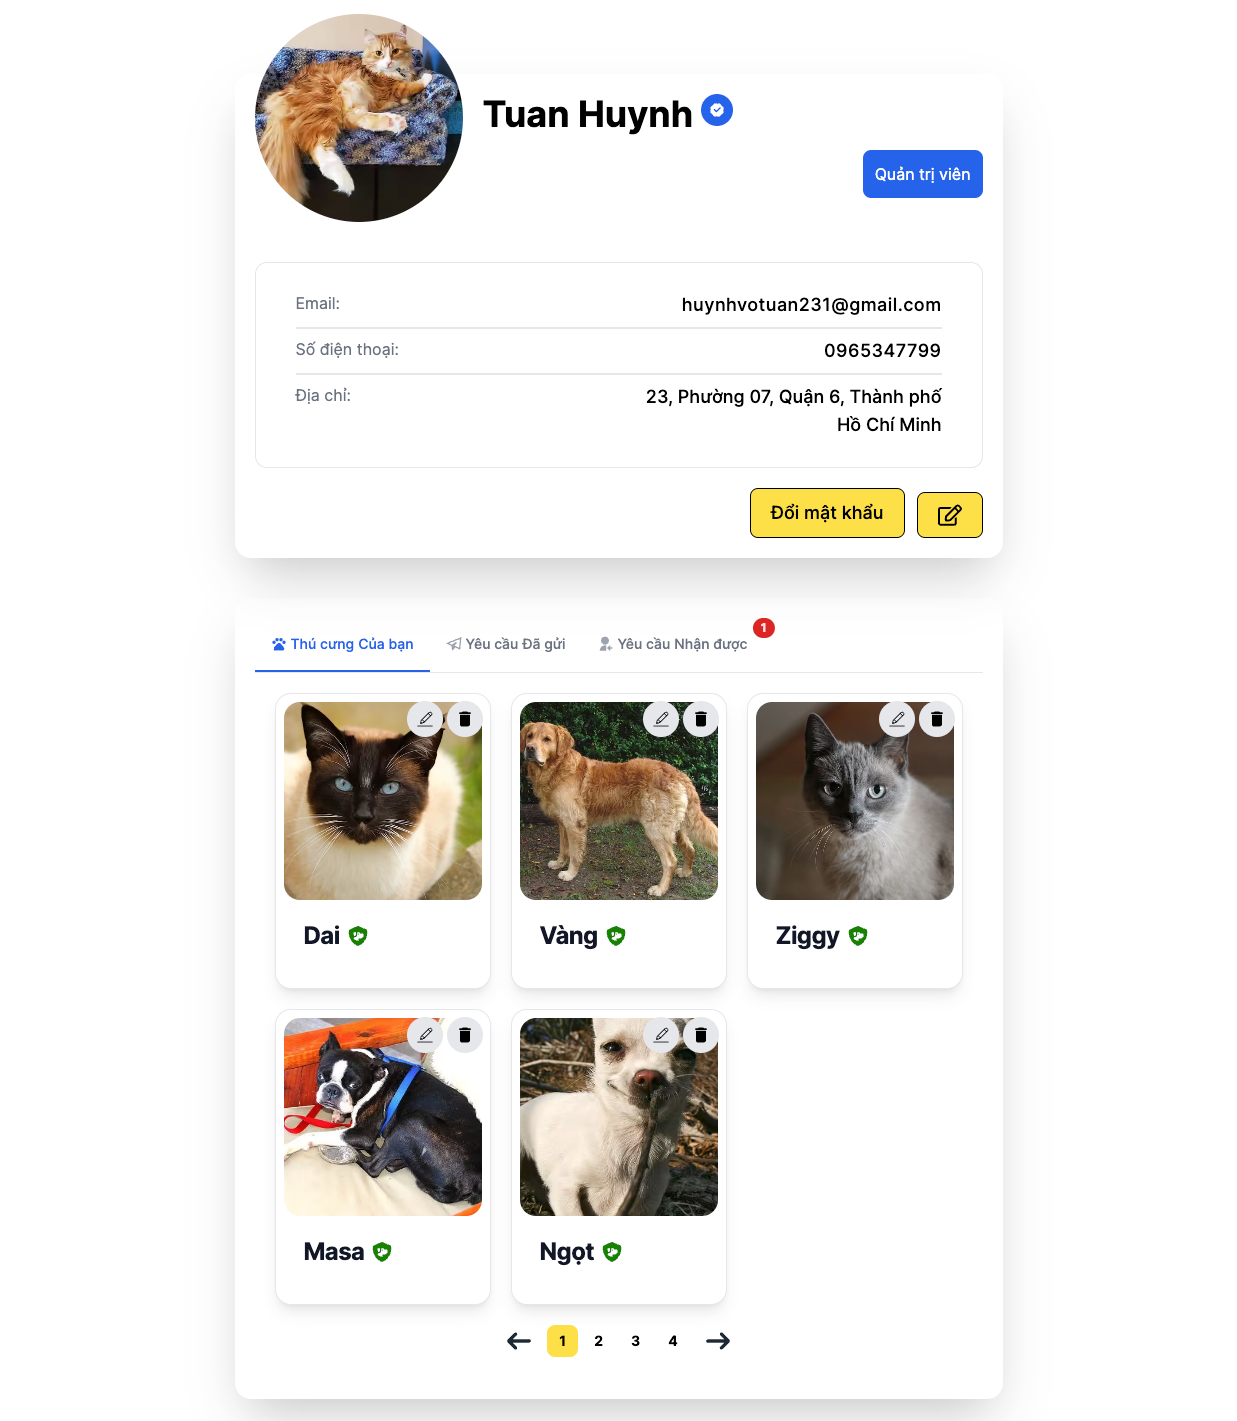
\includegraphics[width=0.7\textwidth]{Figures/UI/user_profile_ui.png}
    \caption{User profile page}
\end{figure}
The user profile page serves as a centralized hub for managing and personalizing 
information, offering a seamless and enjoyable experience. At the top, users will 
find their avatar, name, address, Gmail, and phone number, all of which can be easily 
edited to keep details up-to-date. User can also change their password or update information in this page. The page also features pet profiles, allowing 
users to manage information about their pets effortlessly. Additionally, a management
 table includes tabs for Sent and Incoming messages, notifying users about adoption
  requests and the status of their adoption forms. This intuitive design ensures 
  users can efficiently handle personal information and engage with our platform's
   pet adoption features.

\subsubsection{Organization profile}
\begin{figure}[H]
    \centering
    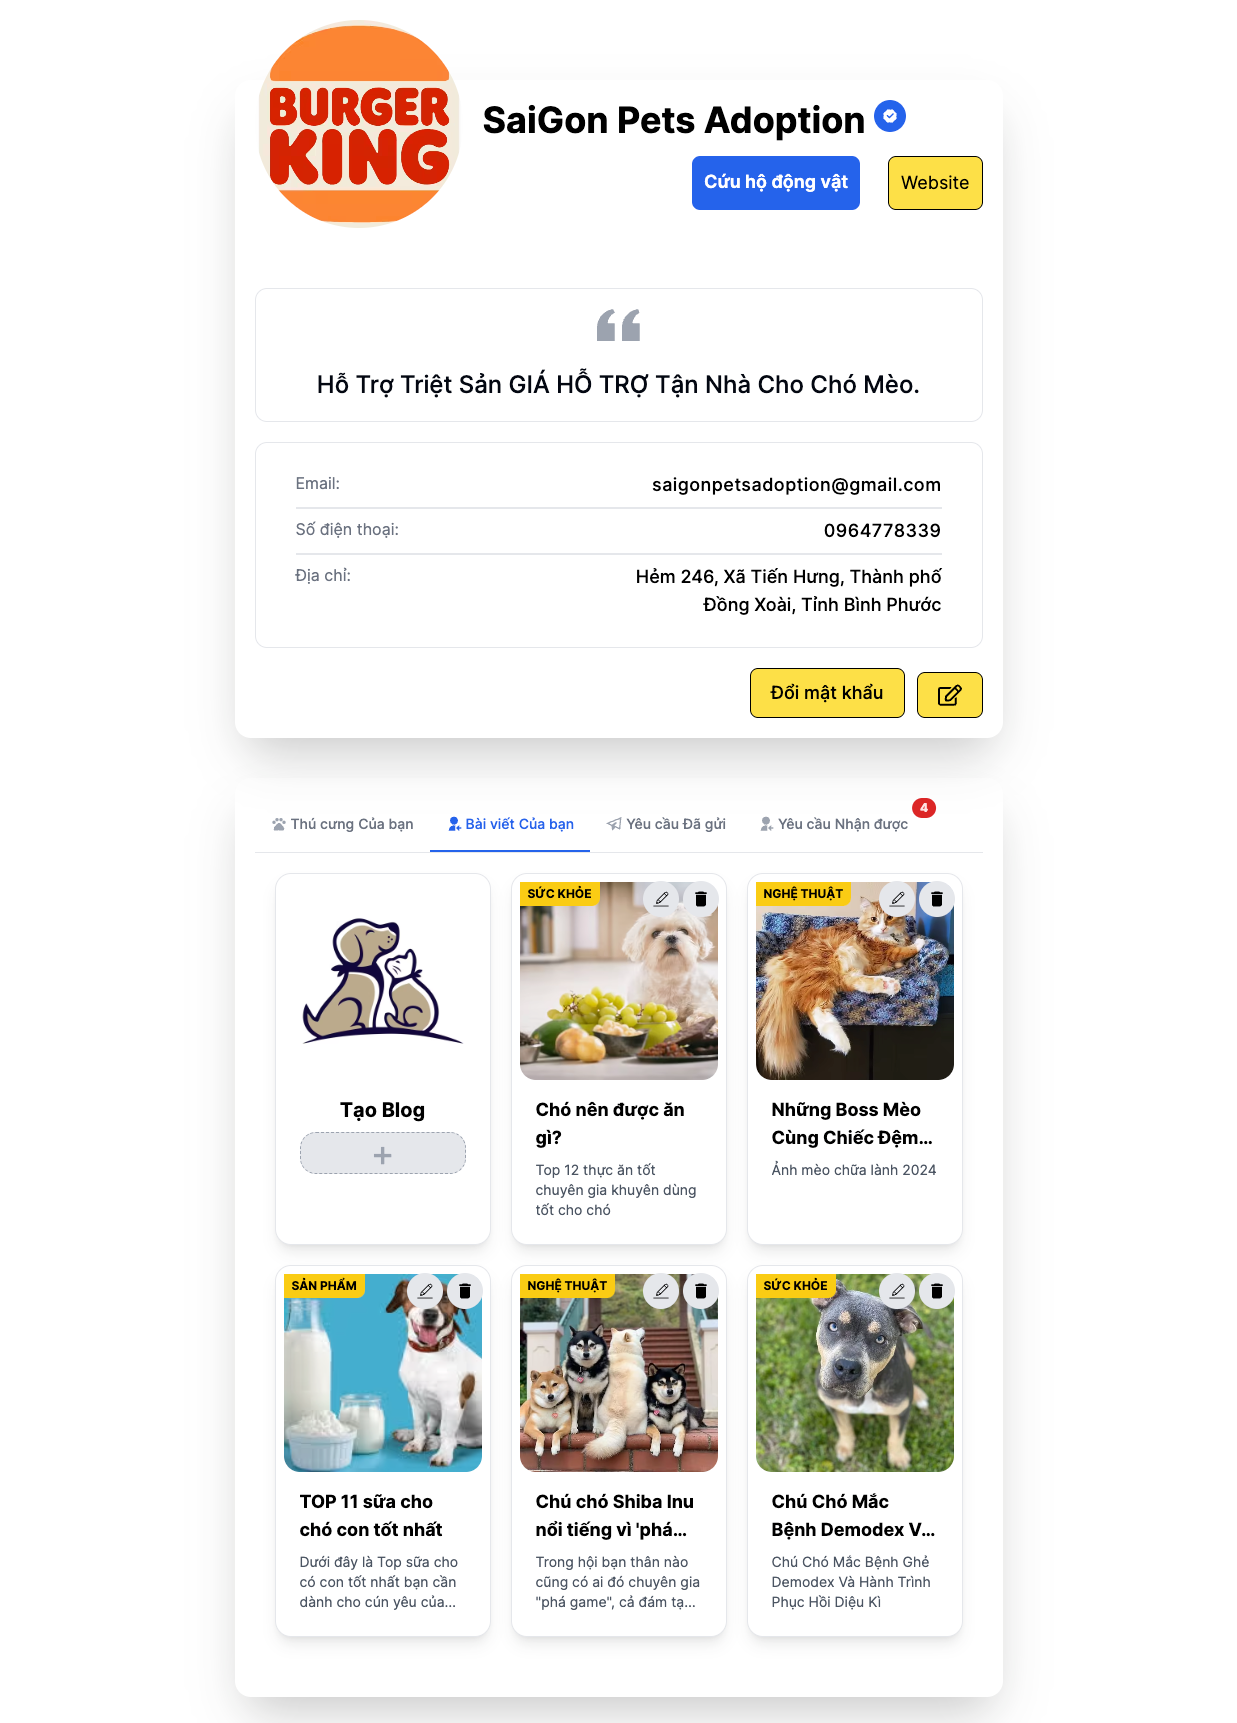
\includegraphics[width=0.7\textwidth]{Figures/UI/org_profile_ui.png}
    \caption{Organization profile page}
\end{figure}

The organization profile mirrors the user profile but includes a verification badge to confirm the account's authenticity. Beneath the organization name, a badge indicates the type of organization. This page also offers functions for changing passwords and updating information. In addition to basic details, the page includes the organization's slogan and web link. The management table features an extra blog tab, allowing users to create, update, or delete blog posts.

\subsubsection{Blog homepage}
\begin{figure}[H]
    \centering
    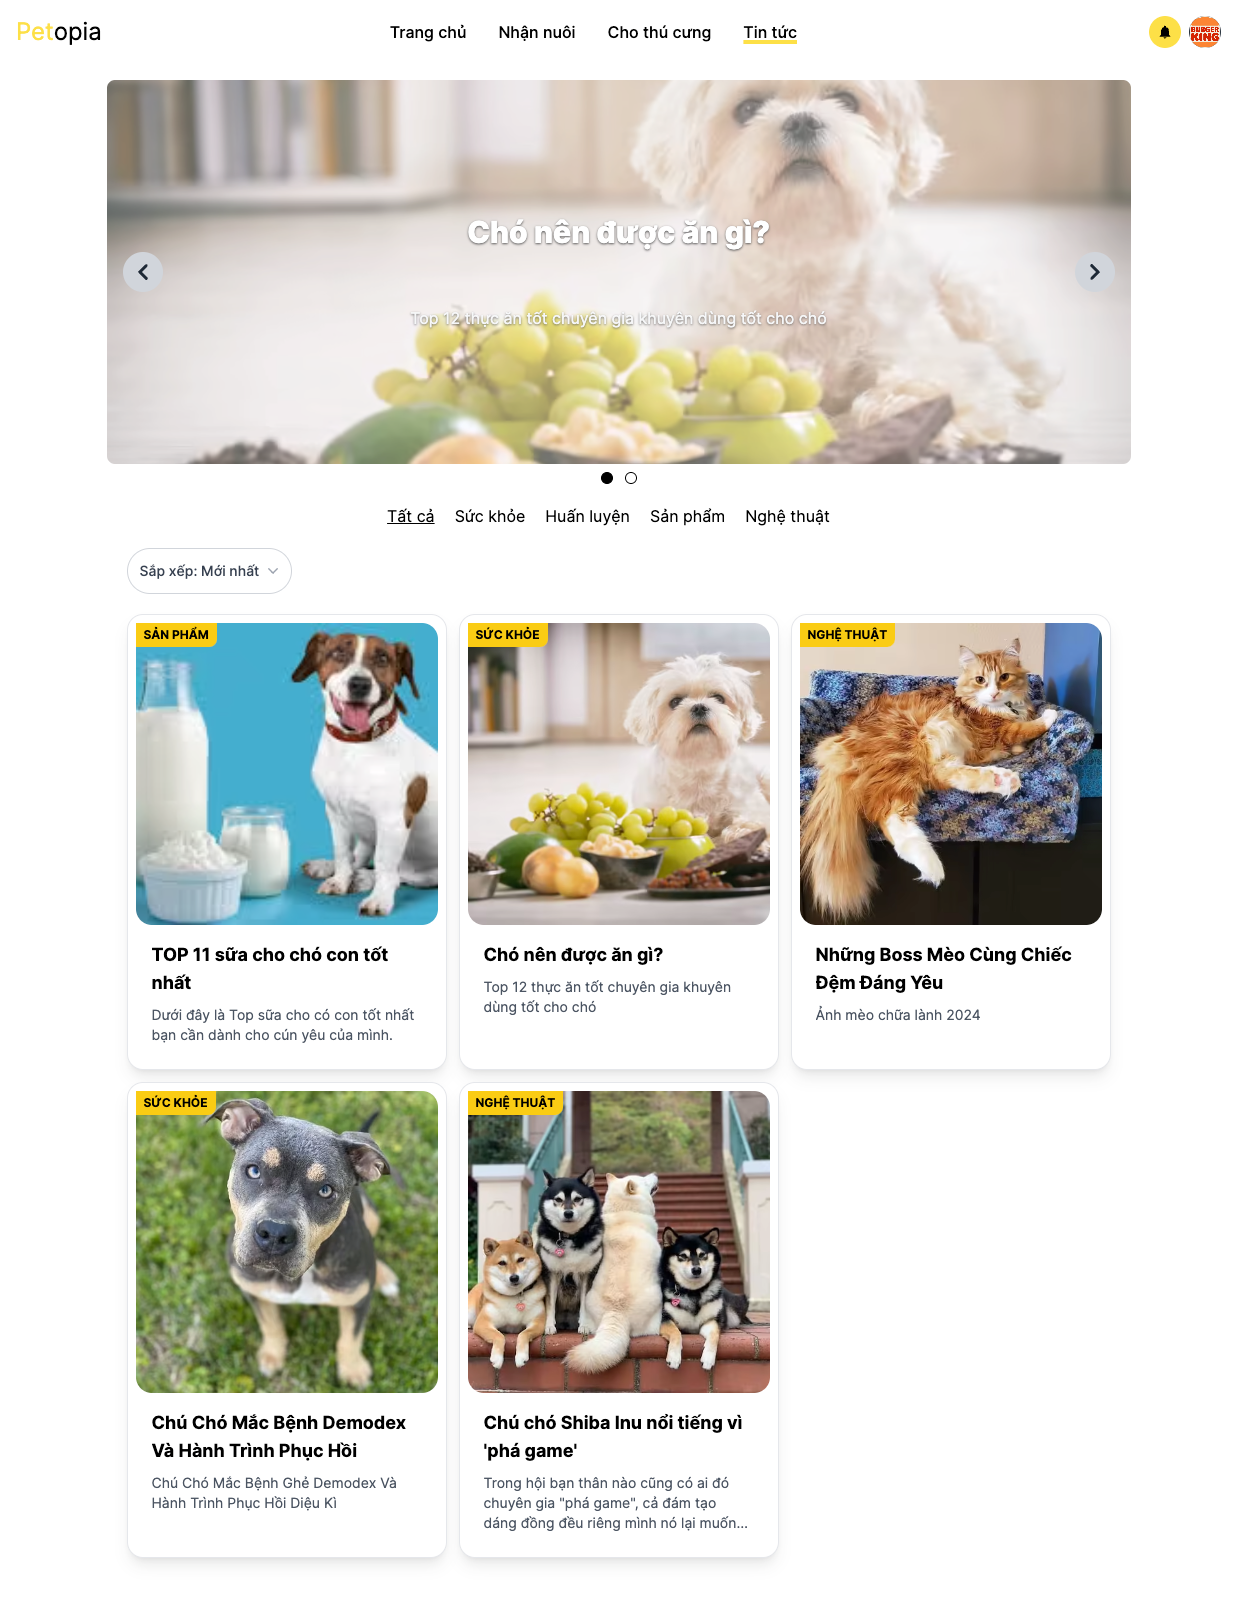
\includegraphics[width=0.8\textwidth]{Figures/UI/blog_ui.png}
    \caption{Blog homepage}
\end{figure}

The blog homepage offers a curated space with various categories for users to explore diverse content.
 Clicking a category dynamically displays relevant blogs, ensuring a targeted reading experience. 
 Selecting a specific blog seamlessly redirects users to the dedicated blog page for detailed 
 exploration. Integrated ads support the platform without disrupting the user experience, 
 contributing to the sustainability of our blog platform.

\subsubsection{Blog page}

\begin{figure}[H]
    \centering
    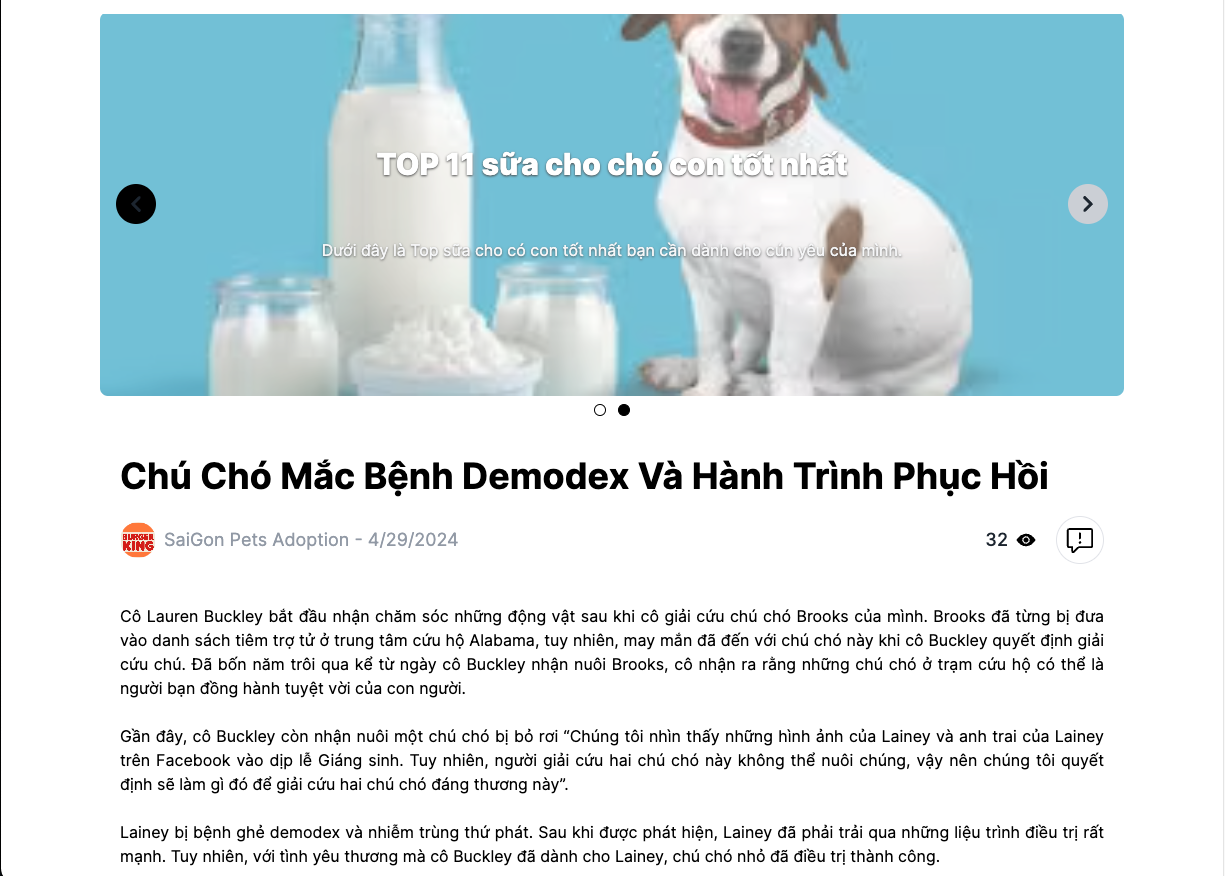
\includegraphics[width=0.8\textwidth]{Figures/UI/blog_page_ui.png}
    \caption{Blog page}
\end{figure}

The blog page ensures a rich and interactive reading experience, allowing users to delve into 
detailed blog posts. Metrics like view count indicate popularity. A relevant section suggests 
related blogs, encouraging users to explore aligned topics for an enhanced and curated experience.

\subsubsection{Payment page}
\begin{figure}[H]
    \centering
    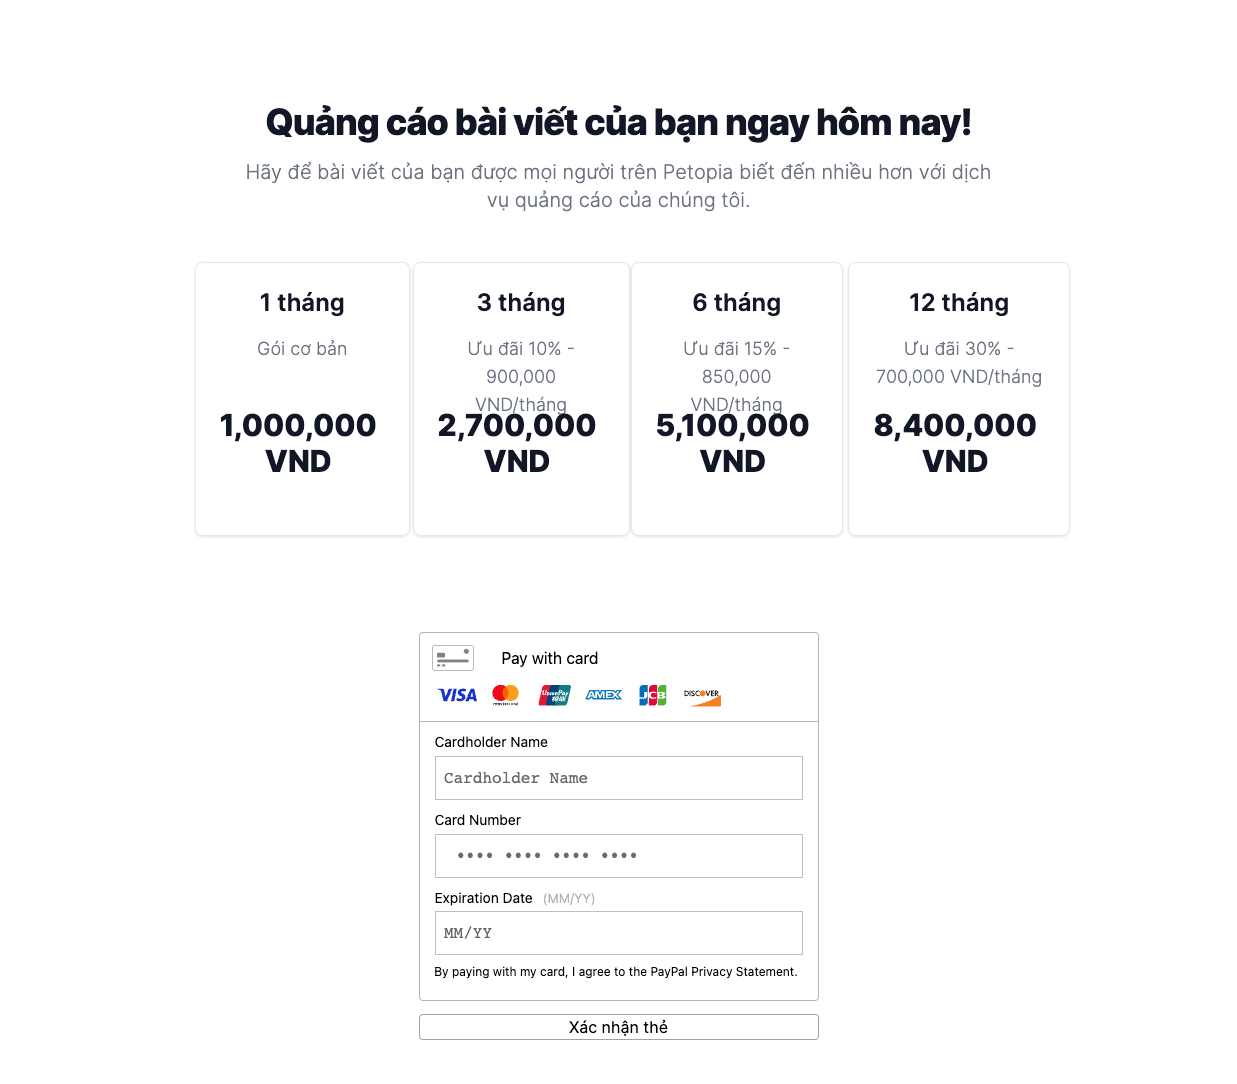
\includegraphics[width=0.8\textwidth]{Figures/UI/payment_ui.png}
    \caption{Payment page}
\end{figure}
On the payment page, users have the option to advertise their blog by selecting from one of four subscription plans: 1 month, 3 months, 6 months, or 12 months. Each plan offers varying levels of exposure and cost, allowing users to choose the duration that best fits their needs and budget. Once a plan is selected, users can proceed by entering their card information in the provided fields. The system ensures secure processing of the payment, after which the advertising plan will be activated. This streamlined process makes it easy for users to promote their blogs effectively.

\newpage
\subsection{Back office}

\subsubsection{Dashboard}

\begin{figure}[H]
    \centering
    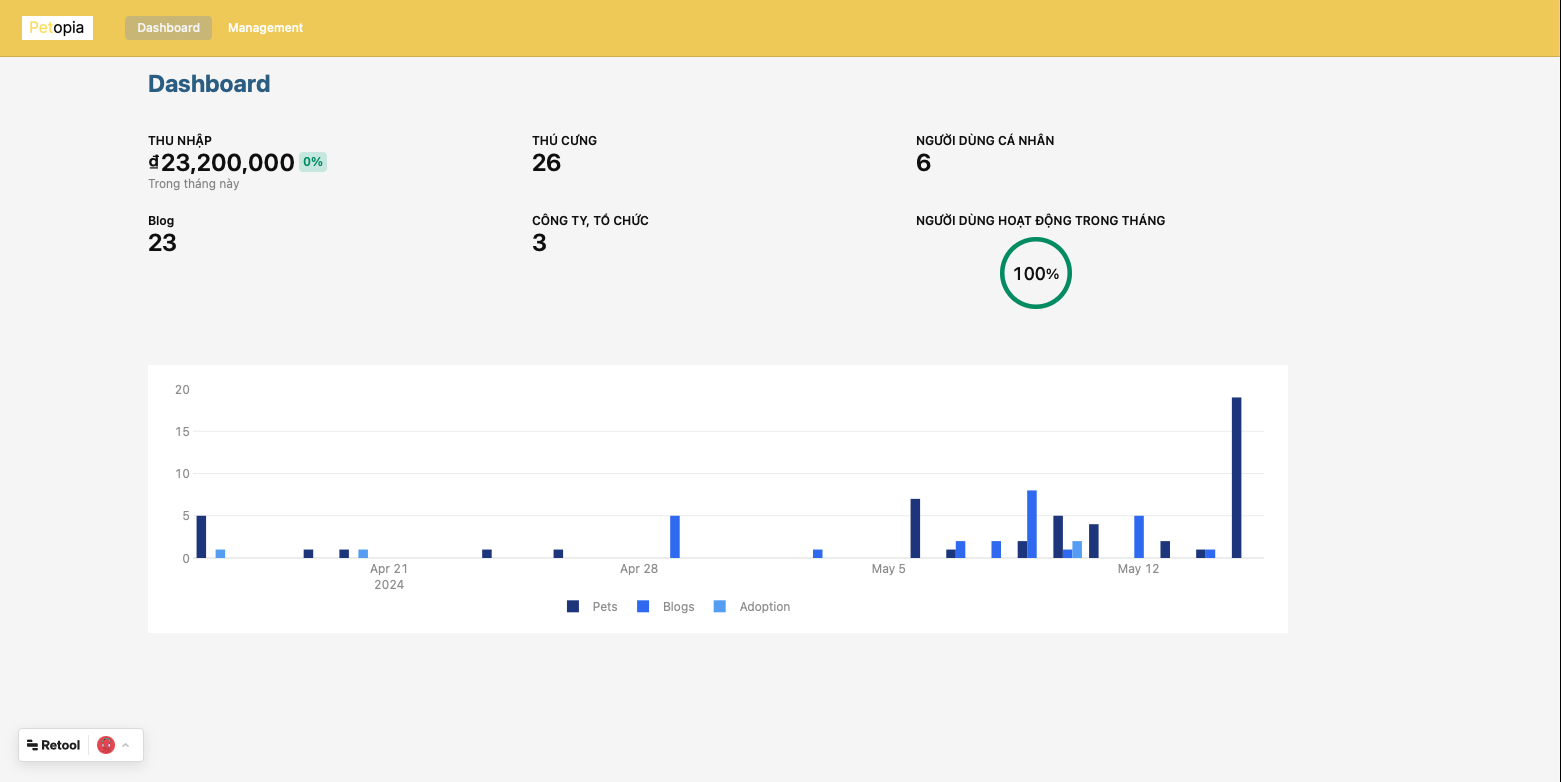
\includegraphics[width=0.7\textwidth]{Figures/UI/dashboard_bo_ui.png}
    \caption{Dashboard to show reports and statistics}
\end{figure}

The dashboard page provides administrators with comprehensive insights into the Petopia website. It displays key metrics such as the number of visitors, pets, blogs, and users. To enhance visualization, graphical representations accompany these statistics, offering a clear and dynamic overview of the platform's performance. This feature allows administrators to efficiently monitor and analyze the website's vital statistics at a glance.

\subsubsection{Control page}

The control page empowers administrators to manage specific data types, including users, blogs, and pets. Administrators can access records, apply filters for efficient navigation, edit fields, enable or disable records, and delete them as needed. This functionality provides administrators with a versatile and centralized tool for comprehensive control and customization of various data records on the platform.

\begin {figure}[H]
\centering
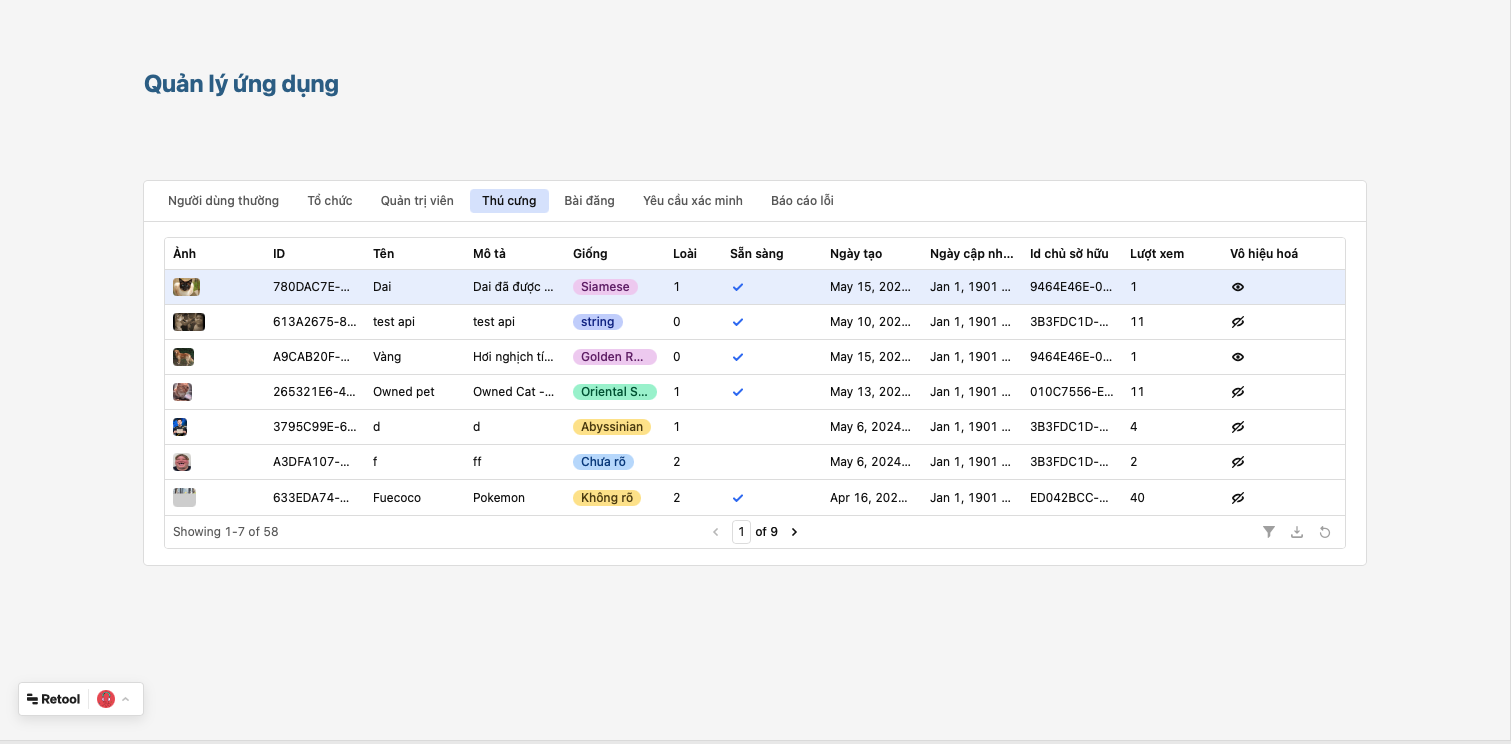
\includegraphics[width=0.7\textwidth]{Figures/UI/control_bo_ui.png}
\caption{Control page for managing data records}
\end{figure}

\newpage
\section{Database design}

\subsection{Conceptual design}

The conceptual design phase of the project is a pivotal stage in the development lifecycle, focused on establishing a comprehensive understanding of the system's structure and relationships.
\\
In \textit{Figure 3.18}, all entities and relationships are presented. Note that all attributes are excluded to enhance visualization and maintain a clear focus on the primary components shaping the system. These attributes will be shown in the physical design section.

\begin{figure}[H]
    \centering
    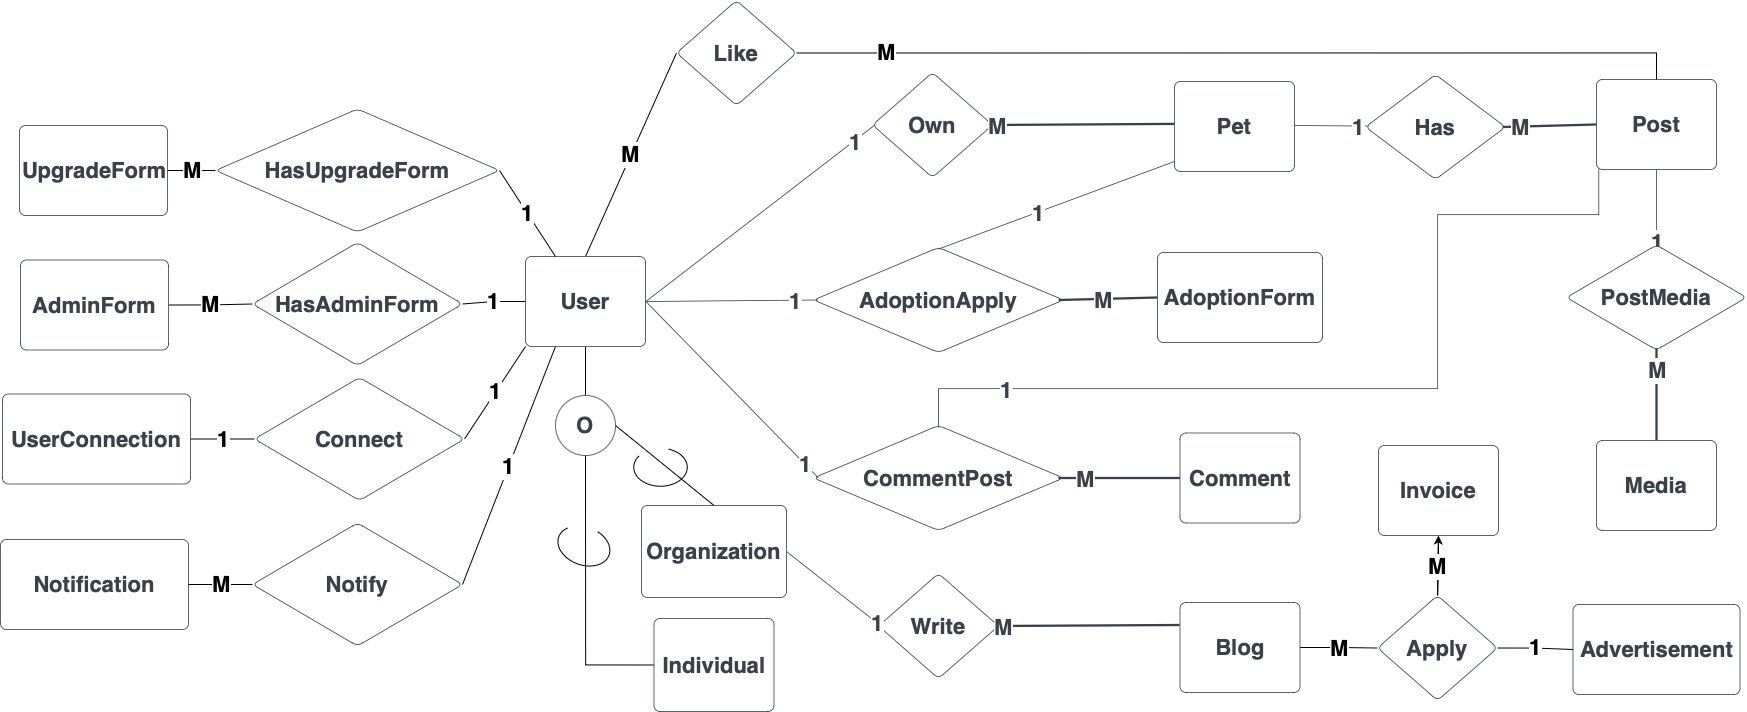
\includegraphics[angle=-90,width=0.4\textwidth]{Figures/DatabaseDesign/Entities-ERD.png}
    \caption{Entity-Relationship diagram}
\end{figure}
\clearpage

\subsection{Relational Design}

In the relational design phase, we use the relational mapping approach
to translate the abstract concepts from the Entity-Relationship Diagram
(ERD) into a concrete relational schema. Through the mapping process,
each entity, along with its attributes and relationships, is
systematically transformed into tables with defined fields and
corresponding constraints in \emph{Figure 3.19}.

\begin {figure}[H]
\centering
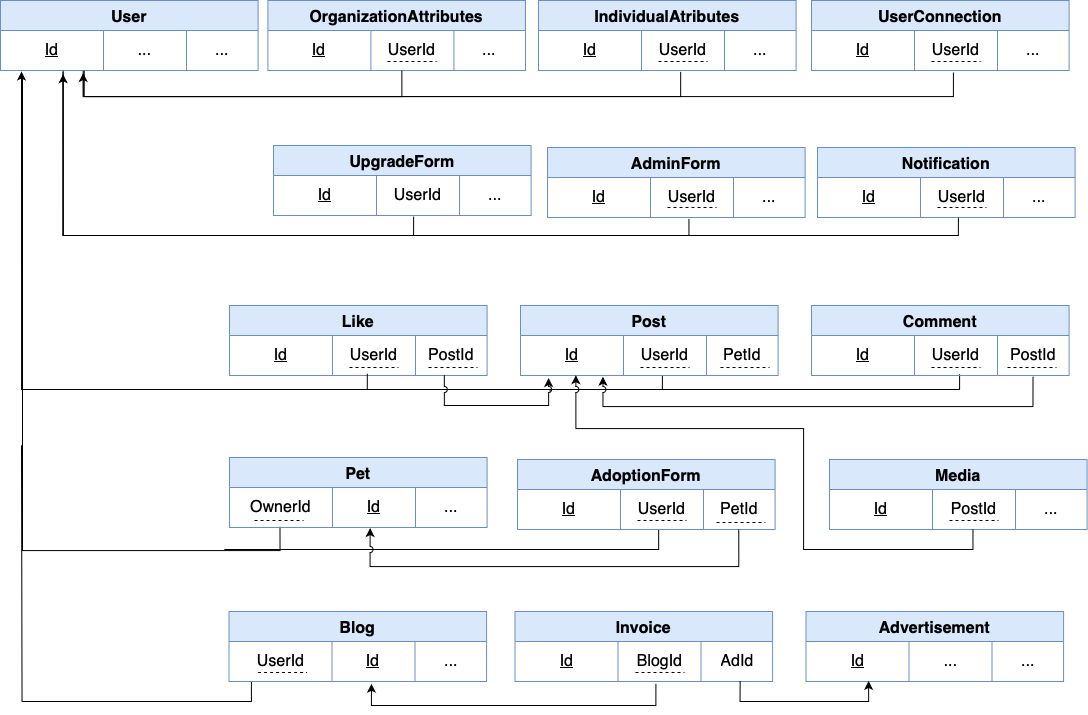
\includegraphics[width=0.9\textwidth]{Figures/DatabaseDesign/Entities-Mapping.png}
\caption{Relational schema}
\end{figure}

\emph{Figure 3.19}, the attributes are not presented fully to ensure a clear visualization of the diagram. In the relational mapping process, we implement a simplified technique for the 3-way relationship where the mandatory entity will take the primary key of the two optional entities as its foreign key, avoiding creating another table causes the schema to become unnecessarily complicated.

\subsection{Physical Design}

In this phase, the conceptual transforms into the tangible, as we build the actual blueprint that mirrors the intricacies of the adoption process in real life. The Relational Schema serves as our guidepost, detailing the tables, and relationships that will form the foundation of the physical database. \textit{Figure 3.20 and 3.21} below translates abstract entities and relationships into concrete data types and optimizes storage structures.

\begin {figure}[H]
\centering
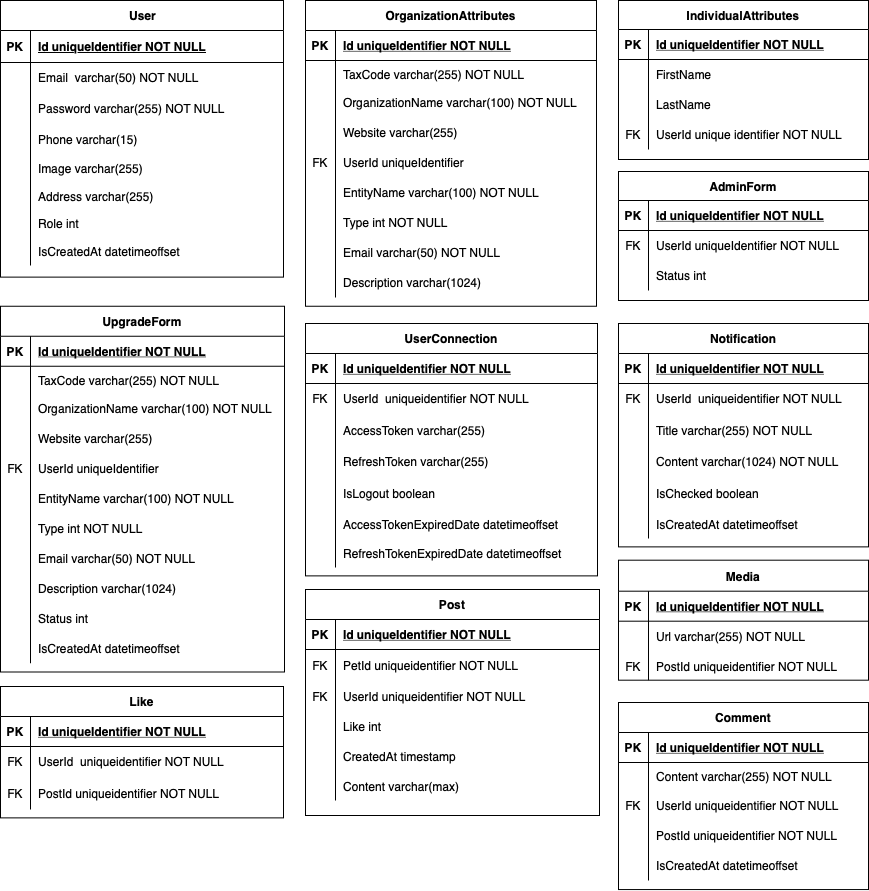
\includegraphics[width=0.8\textwidth]{Figures/DatabaseDesign/Entities-Physical_1.png}
\caption{Physical design}
\end{figure}

\begin {figure}[H]
\centering
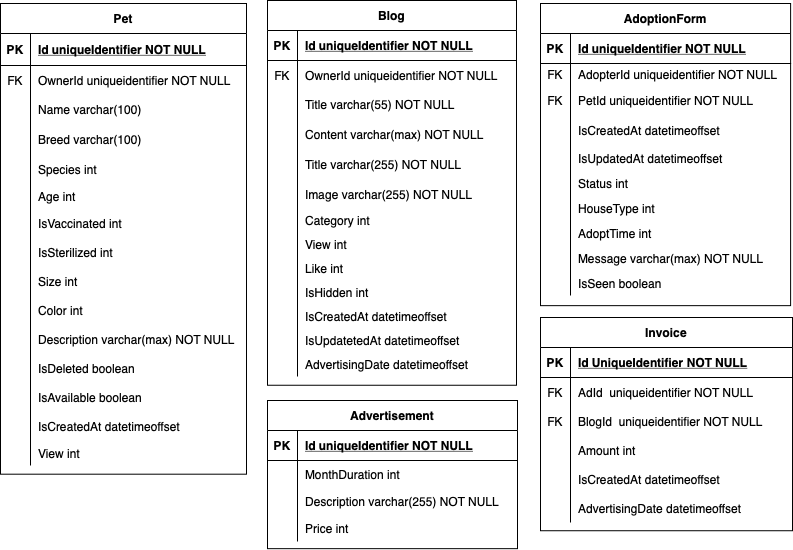
\includegraphics[width=0.8\textwidth]{Figures/DatabaseDesign/Entities-Physical_2.png}
\caption{Physical design (cont)}
\end{figure}






%-	Danh mục TL tham khảo
%-	Phụ lục (nếu có)

% comment two lines and use manually.bbl bellow if manually
\bibliographystyle{plain} % ieeetr
\bibliography{refs} 

% un-comment this line to use manually
% \input{manually.bbl}

\end{document}
